% TEMPLATE for Usenix papers, specifically to meet requirements of
%  USENIX '05
% originally a template for producing IEEE-format articles using LaTeX.
%   written by Matthew Ward, CS Department, Worcester Polytechnic Institute.
% adapted by David Beazley for his excellent SWIG paper in Proceedings,
%   Tcl 96
% turned into a smartass generic template by De Clarke, with thanks to
%   both the above pioneers
% use at your own risk.  Complaints to /dev/null.
% make it two column with no page numbering, default is 10 point

% Munged by Fred Douglis <douglis@research.att.com> 10/97 to separate
% the .sty file from the LaTeX source template, so that people can
% more easily include the .sty file into an existing document.  Also
% changed to more closely follow the style guidelines as represented
% by the Word sample file. 
% This version uses the latex2e styles, not the very ancient 2.09 stuff.
\documentclass[letterpaper,twocolumn,10pt]{article}
\usepackage{usenix,epsfig,endnotes,xspace,color}

% Name candidates:
%  Anza
%  Void 
%  Station (from Genesis's "Grand Central" component) 
%  TARDIS: Atomic, Recoverable, Datamodel Independent Storage
% EAB: flex, basis, stable, dura
% Stasys:  SYStem for Adaptable Transactional Storage: 

\newcommand{\yad}{Stasys\xspace}
\newcommand{\yads}{Stasys'\xspace}
\newcommand{\oasys}{Oasys\xspace}

\newcommand{\eab}[1]{\textcolor{red}{\bf EAB: #1}}
\newcommand{\rcs}[1]{\textcolor{green}{\bf RCS: #1}}
\newcommand{\mjd}[1]{\textcolor{blue}{\bf MJD: #1}}

\newcommand{\eat}[1]{}

\begin{document}

%don't want date printed
\date{}


%make title bold and 14 pt font (Latex default is non-bold, 16 pt)
\title{\Large \bf \yad: System for adapatable, transactional storage}

%for single author (just remove % characters)
\author{
{\rm Russell Sears}\\
UC Berkeley
\and
{\rm Eric Brewer}\\
UC Berkeley
} % end author

\maketitle

% Use the following at camera-ready time to suppress page numbers.
% Comment it out when you first submit the paper for review.
%\thispagestyle{empty}


%\subsection*{Abstract}

{\em There is an increasing need to manage data well in a wide variety of
systems, including robust support for atomic durable concurrent
transactions.  Databases provide the default solution, but force
applications to interact via SQL and to forfeit control over data
layout and access mechanisms.  We argue there is a gap between DBMSs and file systems that limits designers of data-oriented applications.

\yad is a storage framework that incorporates ideas from traditional
write-ahead-logging storage algorithms and file systems,
while providing applications with flexible control over data structures, layout, and performance vs. robustness tradeoffs.
% increased control over their
%underlying modules.  Generic transactional storage systems such as SQL
%and BerkeleyDB serve many applications well, but impose constraints
%that are undesirable to developers of system software and
%high-performance applications.  Conversely, while filesystems place
%few constraints on applications, the do not provide atomicity or
%durability properties that naturally correspond to application needs.

\yad enables the development of
unforeseen variants on transactional storage by generalizing
write-ahead-logging algorithms.  Our partial implementation of these
ideas already provides specialized (and cleaner) semantics to applications.

%Applications may use our modular library of basic data strctures to
%compose new concurrent transactional access methods, or write their
%own from scratch.  

We present examples that make use of custom access methods,
modifed buffer manager semantics, direct log file manipulation, and
LSN-free pages that facilitate zero-copy optimizations, and discuss
the composability of these extensions.

We evaluate the performance of a traditional transactional storage
system based on \yad, and show that it performs comparably to existing
systems.  Application-specific optimizations that can not be expressed
within existing transactional storage implementations allow us to more
than double system performance with little effort.  }

%We argue that our ability to support such a diverse range of
%transactional systems stems directly from our rejection of
%assumptions made by early database designers.  These assumptions
%permeate ``database toolkit'' research.  We attribute the success of
%low-level transaction processing libraries (such as Berkeley DB) to
%a partial break from traditional database dogma.

% entries, and 
% to reduce memory and
%CPU overhead, reorder log entries for increased efficiency, and do
%away with per-page LSNs in order to perform zero-copy transactional
%I/O.  
%We argue that encapsulation allows applications to compose
%extensions.

%These ideas have been partially implemented, and initial performance
%figures, and experience using the library compare favorably with
%existing systems.



\section{Introduction}

As our reliance on computing infrastructure has increased, a wider range of 
applications require robust data management.  Traditionally, data management
has been the province of database management systems (DBMSs), which although
well-suited to enterprise applications, lead to poor support for a
wide-range systems including grid and scientific computing,
bioinformatics, search engines, version control, and workflow
applications.  These applications need transactions but do not fit well
onto SQL and the monolithic approach of current databases.  In
fact, DBMSs are often not used for these systems, which instead
implement custom, ad-hoc data management tools on top of file
systems.

A typical example of this mismatch is in the support for
persistent objects.
% in Java, called {\em Enterprise Java Beans}
%(EJB). 
In a typical usage, an array of objects is made persistent by
mapping each object to a row in a table (or sometimes multiple
tables)~\cite{xxx} and then issuing queries to keep the objects and
rows consistent. A typical update must confirm it has the current
version, modify the object, write out a serialized version using the
SQL update command and commit. This is an awkward and slow mechanism;
we show up to a 5x speedup over a MySQL implementation that is
optimized for single-threaded, local access (Section XXX).

Similarly, bioinformatics systems perform complex scientific
computations over large, semi-structured databases with rapidly evolving schemas.  Versioning and
lineage tracking are also key concerns.  Relational databases support
none of these features well.  Instead, office suites, ad-hoc
text-based formats and Perl scripts are used for data management~\cite{perl, excel}.

\eat{
Examples of real world systems that currently fall into this category
are web search engines, document repositories, large-scale web-email
services, map and trip planning services, ticket reservation systems,
photo and video repositories, bioinformatics, version control systems,
workflow applications, CAD/VLSI applications and directory services.

In short, we believe that a fundamental architectural shift in
transactional storage is necessary before general purpose storage
systems are of practical use to modern applications.
Until this change occurs, databases' imposition of unwanted
abstraction upon their users will restrict system designs and
implementations.
}

%In short, reliable data managment has become as unavoidable as any
%other operating system service.  As this has happened, database
%designs have not incorporated this decade-old lesson from operating
%systems research:
%
%\begin{quote} The defining tragedy of the operating systems community
%  has been the definition of an operating system as software that both
%  multiplexes and {\em abstracts} physical resources...The solution we
%  propose is simple: complete elimination of operating sytems
%  abstractions by lowering the operating system interface to the
%  hardware level~\cite{engler95}.
%\end{quote}

The widespread success of lower-level transactional storage libraries
(such as Berkeley DB) is a sign of these trends.  However, the level
of abstraction provided by these systems is well above the hardware
level, and applications that resort to ad-hoc storage mechanisms are
still common.

This paper presents \yad, a library that provides transactional
storage at a level of abstraction as close to the hardware as
possible.  The library can support special purpose, transactional
storage interfaces as well as ACID database-style interfaces to
abstract data models.  \yad incororates techniques from the databases
(e.g. write-ahead logging) and systems (e.g. zero-copy techniques).
Our goal is to combine the flexibility and layering of low-level
abstractions typical for systems work, with the complete semantics
that exemplify the database field.

By {\em flexible} we mean that \yad{}  can implement a wide
range of transactional data structures, that it can support a variety
of policies for locking, commit, clusters and buffer management.
Also, it is extensible for both new core operations
and new data structures. It is this flexibility that allows the
support of a wide range of systems.

By {\em complete} we mean full redo/undo logging that supports
both {\em no force}, which provides durability with only log writes,
and {\em steal}, which allows dirty pages to be written out prematurely
to reduce memory pressure. By complete, we also
mean support for media recovery, which is the ability to roll
forward from an archived copy, and support for error-handling,
clusters, and multithreading. These requirements are difficult
to meet and form the {\em raison d'\^etre} for \yad{}: the framework
delivers these properties as reusable building blocks for systems
to implement complete transactions.

Through examples, and their good performance, we show how \yad{}
support a wide range of uses that in the database gap, including
persistent objects (roadmap?), graph or XML apps, and recoverable
virtual memory~\cite{lrvm}.  An (early) open-source implementation of
the ideas presented below is available.

\eab{others?  CVS, windows registry, berk DB, Grid FS?}

roadmap?



\section{\yad is not a Database}

Database research has a long history, including the development of
many technologies that our system builds upon.  This section explains
why databases are fundamentally inappropriate tools for system
developers.  The problems we present here have been the focus of
database systems and research projects for at least 25 years.

The section concludes with a discussion of database systems that
attempt to address these problems.  Although these systems were
successful in many respects, they fundamentally aim to implement a
data model, rather than build transactions from the bottom up. \eab{move this?}


\subsection{The database abstraction}

Database systems are often thought of in terms of the high-level
abstractions they present.  For instance, relational database systems
implement the relational model~\cite{cobb}, object oriented
databases implement object abstractions, XML databases implement
hierarchical datasets, and so on.  Before the relational model,
navigational databases implemented pointer- and record-based data models.

An early survey of database implementations sought to enumerate the
fundamental components used by database system implementors.  This
survey was performed due to difficulties in extending database systems
into new application domains.  The survey divided internal database
routines into two broad modules: {\em conceptual
mappings}~\cite{batoryConceptual} and the {\em physical
database}~\cite{batoryPhysical} model.

A conceptual mapping might translate a relation into a set of keyed
tuples.  A physical model would then translate a set of tuples into an
on-disk B-Tree, and provide support for iterators and range-based query
operations.

It is the responsibility of a database implementor to choose a set of
conceptual mappings that implement the desired higher-level
abstraction (such as the relational model).  The physical data model
is chosen to efficiently support the set of mappings that are built on
top of it.

{\em A key observation of this paper is that no known physical data model
can support more than a small percentage of today's applications.}

Instead of attempting to create such a model after decades of database
research has failed to produce one, we opt to provide a transactional
storage model that mimics the primitives provided by modern hardware.
This makes it easy for system designers to implement most of the data
models that the underlying hardware can support, or to
abandon the data model approach entirely, and forgo the use of a
structured physical model or conceptual mappings.

\subsection{Extensible databases}

Genesis~\cite{genesis}, an early database toolkit, was built in terms
of a physical data model, and the conceptual mappings desribed above.
It was designed allow database implementors to easily swap out
implementations of the various components defined by its framework.
Like subsequent systems (including \yad), it allowed it users to
implement custom operations.

Subsequent extensible database work builds upon these foundations.
For example, the Exodus~\cite{exodus} database toolkit was the successor to
Genesis. It supported the autmatic generation of query optimizers and
execution engines based upon abstract data type definitions, access
methods and cost models provided by its users.

\eab{move this next paragraph to RW?}

Starburst's~\cite{starburst} physical data model consisted of {\em
  storage methods}.  Storage methods supported {\em attachment types}
that allowed triggers and active databases to be implemented.  An
attachment type is associated with some data on disk, and is invoked
via an event queue whenever the data is modified.  In addition to
providing triggers, it was used to facilitate index management.
Starburst includes a type system that supported multiple inheritance,
and it supports hints such as information regarding desired physical
clustering.  Starburst also included a query language.

Although further discussion is beyond the scope of this paper,
object-oriented database systems, and relational databases with
support for user-definable abstract data types (such as in
Postgres~\cite{postgres}) were the primary competitors to extensible
database toolkits.  Ideas from all of these systems have been
incorporated into the mechanisms that support user-definable types in
current database systems.

One can characterise the difference between database toolkits and
extensible database servers in terms of early and late binding.  With
a database toolkit, new types are defined when the database server is
compiled.  In today's object-relational database systems, new types
are defined at runtime.  Each approach has its advantages.  However,
both types of systems aim to extend a high-level data model with new abstract data types, and thus are quite limited in the range of new applications they support.  Not surprisingly, this kind of extensibility has had little impact on the range of applications we listed above.

\subsection{Berkeley DB}

System R was the first relational database implementation, and was
based upon a clean separation between its storage system and its
query processing engine.  In fact, it supported a simple navigational
interface to the storage subsystem.  To this day, database systems are
built using this sort of architecture.  

Berkeley DB is a highly successful alternative to conventional
database design.  At its core, it provides the physical database, or
the relational storage system of a conventional database server.
It is based on the
observation that the storge subsystem is a more general (and less
abstract) component than a monolithic database, and provides a
standalone implementation of the storage primitives built into 
most relational database systems~\cite{libtp}.  In particular, 
it provides fully transactional (ACID) operations over B-Trees, 
hashtables, and other access methods.  It provides flags that 
let its users tweak various aspects of the performance of these
primitives.

We have already discussed the limitations of this approach.  With the
exception of the direct comparison of the two systems, none of the \yad 
applications presented in Section~\ref{extensions} are efficiently
supported by Berkeley DB.   This is a result of Berkeley DB's  
assumptions regarding workloads and decisions regarding low level data
representation.  Thus, although Berkeley DB could be built on top of \yad,
Berkeley DB is too specialized to support \yad.

\eab{for BDB, should we say that it still has a data model?}



%cover P2 (the old one, not "Pier 2" if there is time...

\subsection{Better databases}

The database community is also aware of this gap. 
A recent survey~\cite{riscDB} enumerates problems that plague users of
state-of-the-art database systems, and finds that database implementations fail to support the
needs of modern systems.  In large systems, this manifests itself as
managability and tuning issues that prevent databases from predictably
servicing diverse, large scale, declartive, workloads.  
On small devices, footprint, predictable performance, and power consumption are
primary, concerns that database systems do not address.

%Midsize deployments, such as desktop installations, must run without
%user intervention, but self-tuning, self-administering database
%servers are still an area of active research.

The survey argues that these problems cannot be adequately addressed without a fundamental shift in the architectures that underly database systems.  Complete, modern database
implementations are generally incomprehensible and
irreproducable, hindering further research.  The study concludes 
by suggesting the adoption of ``RISC''-style database architectures, both as a research and an
implementation tool~\cite{riscDB}.  

RISC databases have many elements in common with
database toolkits.  However, they take the database toolkit idea one
step further, and suggest standardizing the interfaces of the
toolkit's internal components, allowing multiple organizations to
compete to improve each module.  The idea is to produce a research
platform, and to address issues that affect modern
databases, such as automatic performance tuning, and reducing the
effort required to implement a new database system~\cite{riscDB}.

We agree with the motivations behind RISC databases, and that a need
for improvement in database technology exists.  In fact, is our hope
that our system will mature to the point where it can support
a competitive relational database.  However this is
not our primary goal.  
Instead, we are interested in supporting applications that derive
little benefit from database abstractions, but that need reliable
storage.  Therefore, instead of building a modular database, we seek
to build a system that enables a wider range of data management options.

%For example, large scale application such as web search, map services,
%e-mail use databases to store unstructured binary data, if at all.

%More recently, WinFS, Microsoft's database based
%file metadata management system, has been replaced in favor of an
%embedded indexing engine that imposes less structure (and provides
%fewer consistency guarantees) than the original
%proposal~\cite{needtocitesomething}.

%Scaling to the very large doesn't work (SAP used DB2 as a hash table
%for years), search engines, cad/vlsi didn't happen.  scalable GIS
%systems use shredded blobs (terraserver, google maps), scaling to many
%was more difficult than implementing from scratch (winfs), scaling
%down doesn't work (variance in performance, footprint),


\section{Transactional Pages}

Section~\ref{notDB} described the ways in which a top-down data model
limits the generality and flexibility of databases.  In this section,
we cover the basic bottom-up approach of \yad: {\em transactional
pages}. Although similar to the underlying write-ahead logging
approaches of databases, particularly ARIES~\cite{aries}, \yads
bottom-up approach yields unexpected flexibility.

Transactional pages provide the properties of transactions, but
limited to updates within a single page in the simplest case.  After
covering the single-page case, we explore multi-page transactions,
which enable a complete transaction system.

In this model, pages are the in-memory representation of disk blocks
and thus must be the same size.  Pages are a convenient abstraction
because the write back of a page (disk block) is normally atomic,
giving us a foundation for larger atomic actions. In practice, disk
blocks are not always atomic, but the disk can detect partial writes
via checksums.  Thus, we actually depend only on detection of
non-atomicity, which we treat as media failure.  One nice property of
\yad is that we can roll forward an individual page from an archive copy to
recover from media failures.

A subtlety of transactional pages is that they technically only
provide the "atomicity" and "durability" of ACID
transactions.\footnote{The "A" in ACID really means atomic persistence
of data, rather than atomic in-memory updates, as the term is normally
used in systems work~\cite{GR97}; the latter is covered by "C" and
"I".}  This is because "isolation" comes typically from locking, which
is a higher (but compatible) layer. "Consistency" is less well defined
but comes in part from transactional pages (from mutexes to avoid race
conditions), and in part from higher layers (e.g. unique key
requirements). To support these, \yad distinguishes between {\em
latches} and {\em locks}.  A latch corresponds to an OS mutex, and is
held for a short period of time.  All of \yads default data structures
use latches and with ordering to avoid deadlock. This allows
multithreaded code to treat \yad as a normal, reentrant data structure
library.  Applications that want conventional isolation
(serializability) use a lock manager above transactional pages.

\eat{
\yad uses write-ahead-logging to support the
four properties of transactional storage: Atomicity, Consistency,
Isolation and Durability.  Like existing transactional storage sytems,
\yad allows applications to disable or choose different variants of each
property.

However, \yad takes customization of transactional semantics one step
further, allowing applications to add support for transactional
semantics that we have not anticipated.  We do not believe that
we can anticipate every possible variation of write ahead logging.  
However, we
have observed that most changes that we are interested in making
involve a few common underlying primitives.  

As we have
implemented new extensions, we have located portions of the system
that are prone to change, and have extended the API accordingly.  Our
goal is to allow applications to implement their own modules to
replace our implementations of each of the major write ahead logging
components.
}


\subsection{Single-page Transactions}

In this section we show how to implement single-page transactions.
This is not at all novel, and is in fact based on ARIES, but it forms
important background.  We also gloss over many important and
well-known optimizations that \yad exploits, such as group
commit~\cite{group-commit}.

The trivial way to acheive single-page transactions is simply to apply
all the updates to the page and then write it out on commit. The page
must be pinned until the transaction commits to avoid "dirty" data
(uncommitted data on disk), but no logging is required.  As disk
block writes are atomic, this ensures that we provide the "A" and "D"
of ACID.

This approach has poor performance since we must {\em force} pages to disk
on commit and wait for a (random access) synchronous write to
complete. By using a write-ahead log, we can support {\em no force}
transactions: we write "redo" information to the log on commit, and
then can write the pages later. If we crash, we can use the log to
redo the lost updates during recovery.

For this to work, we need to be able to tell which updates to
re-apply, which is solved by using a per-page sequence number called a
{\em log sequence number}. Each log entry contains the sequence
number, and each page contains the sequence number of the last applied
update.  Thus on recovery, we load a page, look at its sequence
number, and re-apply all later updates.  Similarly, to restore a page
from archive we use the same process, but with likely many more
updates to apply.

We also need to make sure we only re-apply updates for transactions
that committed.  This is best done by writing a commit record to the
log during the commit.  Transactions without commit records should not
be recovered.

Pinning the pages of active transactions leads to problems as well.
First, a single transaction may need more pages than can be pinned at
one time. Second, under concurrent transactions, a given page may be
pinned forever as long as it has at least one active transaction in
progress all the time.  To avoid these problems, transaction systems
support a {\em steal}, which means that pages can be written back
before a transaction commits. 

Thus, on recovery a page may contain data that never committed and the
corresponding updates must be rolled back.  To enable this, "undo" log
entries for uncommitted updates must be on disk before the page can be
stolen (written back).  On recovery, the LSN on the page reveals which
UNDO entries to apply to roll back the page. We use the absence of
commit records to figure out which transactions to roll back.

Thus, the single-page transactions of \yad work as follows.  An {\em
operation} consists of both a redo and an undo function, both of which
take one argument. An update is always the redo function applied to
the page (there is no "do" function), and it always ensures that the
redo log entry (with its LSN and argument) reach the disk before
commit.  Similarly, an undo log entry, with its LSN and argument,
alway reaches the disk before a page is stolen.  ARIES works
essentially the same way, but without the ability to easily add new
operations.

To manually abort a transaction, the \yad could either reload the page
from disk and roll it forward to reflect committed transactions, or it
could roll back the page using the undo entries applied in reverse LSN
order. (It currently does the latter.)


\eat{
Write ahead logging algorithms are quite simple if each operation
applied to the page file can be applied atomically.  This section will
describe a write ahead logging scheme that can transactionally update
a single page of storage that is guaranteed to be written to disk
atomically.  We refer the readers to the large body of literature
discussing write ahead logging if more detail is required.  Also, for
brevity, this section glosses over many standard write ahead logging
optimizations that \yad implements.


Assume an application wishes to transactionally apply a series of
functions to a piece of persistant storage.  For simplicity, we will
assume we have two deterministic functions, {\em undo}, and {\em
redo}.  Both functions take the contents of a page and a second
argument, and return a modified page.

As long as their second arguments match, undo and redo are inverses of
each other.  Normally, only calls to abort and recovery will invoke undo, so
we will assume that transactions consist of repeated applications of
the redo function.

Following the lead of ARIES (the write ahead logging system \yad
originally set out to implement), assume that the function is also
passed a distinct, monotonically increasing number each time it is
invoked, and that it records that number in an LSN (log sequence number)
field of the page.  In section~\ref{lsnFree}, we do away with this requirement.

We assume that while undo and redo are being executed, the
page they are modifying is pinned in memory.  Between invocations of
the two functions, the write-ahead-logging system may write the page
back to disk.  Also, multiple transactions may be interleaved, but
undo and redo must be executed atomically.  (However, \yad supports concurrent execution of operations.)

Finally, we assume that each invocation of redo and undo is recorded
in the log, along with a transaction id, LSN, and the argument passed into the redo or undo function.
(For efficiency, the page contents are not stored in the log.)

If abort is called during normal operation, the system will iterate
backwards over the log, invoking undo once for each invocation of redo
performed by the aborted transaction.  It should be clear that, in the
single transaction case, abort will restore the page to the state it
was in before the transaction began.  Note that each call to undo is
assigned a new LSN so the page LSN will be different.  Also, each undo
is also written to the log.
}

\eab{describe recovery?}

Recovery is handled by playing the log forward, and only applying log
entries that are newer than the version of the page on disk.  Once the
end of the log is reached, recovery proceeds to abort any transactions
that did not commit before the system crashed.\endnote{Like ARIES,
\yad actually implements recovery in three phases, Analysis, Redo and
Undo.}  Recovery arranges to continue any outstanding aborts where
they left off, instead of rolling back the abort, only to restart it
again.

\eat{
Note that recovery relies on the fact that it knows which version of
the page is recorded on disk, and that the page itself is
self-consistent.  If it passes an unknown version of a page into undo
(which is an arbitrary function), it has no way of predicting what
will happen.
}


\subsection{Multi-page transactions}

Of course, in practice, we wish to support transactions that span more
than one page.  Given a no-force/steal single-page transaction, this
is relatively easy.

First, we need to ensure that all log entries have a transaction ID
(XID) so that we can tell that updates to different pages are part of
the same transaction (we need this for multiple updates within a
single page too).  Given single-page recovery, we can just apply it to
all of the pages touched by a transaction to recover a multi-page
transaction.  This works because steal and no-force already imply
that pages can be written back early or late (respectively), so there
is no need to write a group of pages back atomically.  In fact, we
need only ensure that redo entries for all pages reach the disk before
the commit record (and before commit returns).

\eat{
\subsection{Write ahead logging invariants}

In order to support recovery, a write-ahead-logging algorithm must
identify pages that {\em may} be written back to disk, and those that
{\em must} be written back to disk.  \yad provides full support for
Steal/no-Force write ahead logging, due to its generally favorable
performance properties.  ``Steal'' refers to the fact that pages may
be written back to disk before a transaction completes.  ``No-Force''
means that a transaction may commit before the pages it modified are
written back to disk.  

In a Steal/no-Force system, a page may be written to disk once the log
entries corresponding to the udpates it contains are written to the
log file.  A page must be written to disk if the log file is full, and
the version of the page on disk is so old that deleting the beginning
of the log would lose redo information that may be needed at recovery.

Steal is desirable because it allows a single transaction to modify
more data than is present in memory.  Also, it provides more
opportunities for the buffer manager to write pages back to disk.
Otherwise, in the face of concurrent transactions that all modify the
same page, it may never be legal to write the page back to disk.  Of
course, if these problems would never come up in practice, an
application could opt for a no-Steal policy, possibly allowing it to
write less undo information to the log file.

No-Force is often desirable for two reasons.  First, forcing pages
modified by a transaction to disk can be extremely slow if the updates
are not near each other on disk.  Second, if many transactions update
a page, Force could cause that page to be written once for each transaction
that touched the page.  However, a Force policy could reduce the
amount of redo information that must be written to the log file.
}


\subsection{Nested top actions}

So far, we have glossed over the behavior of our system when multiple
transactions execute concurrently.  To understand the problems that
can arise when multiple transactions run concurrently, consider what
would happen if one transaction, A, rearranged the layout of a data
structure.  Next, assume a second transaction, B, modified that
structure, and then A aborted.  When A rolls back, its UNDO entries
will undo the rearrangment that it made to the data structure, without
regard to B's modifications.  This is likely to cause corruption.

Two common solutions to this problem are ``total isolation'' and
``nested top actions.''  Total isolation simply prevents any
transaction from accessing a data structure that has been modified by
another in-progress transaction.  An application can achieve this
using its own concurrency control mechanisms, or by holding a lock on
each data structure until the end of the transaction.  Releasing the
lock after the modification, but before the end of the transaction,
increases concurrency but means that follow-on transactions that use
that data likely need to abort if the current transaction aborts ({\em
cascading aborts}.

Unfortunately, total isolation causes bottlenecks when applied to key
data structures, since the structure is locked for a relatively long
time.  Nested top actions are essentially mini-transactions that can
commit even if their containing transaction aborts; thus follow-on
transactions can use the data structure without fear of cascading
aborts.  

The key idea is to distinguish between the logical operations of a
data structure, such as inserting a key, and the physical operations
such as splitting tree nodes or or rebalancing a tree. These physical
operations do not need to undone if the containing logical operation
(insert) aborts.

Because nested top actions are easy to use and do not lead to 
deadlock, we wrote a simple \yad extension that
implements nested top actions.  The extension may be used as follows:

\begin{enumerate}
\item Wrap a mutex around each operation.  With care, it may be possible to use finer-grained locks, but it is rarely necessary.
\item Define a {\em logical} UNDO for each operation (rather than just using
  a set of page-level UNDO's).  For example, this is easy for a
  hashtable: the UNDO for {\em insert} is {\em remove}.
\item For mutating operations, (not read-only), add a ``begin nested
  top action'' right after the mutex acquisition, and a ``commit
  nested top action'' right before the mutex is released.
\end{enumerate}

If the transaction that encloses the operation aborts, the logical
undo will {\em compensate} for its effects, leaving the structural
changes intact.  Note that this recipe does not ensure transactional
consistency and is largely orthogonol to the use of a lock manager.

We have found that it is easy to protect operations that make
structural changes to data structures with this recipe.
Therefore, we use them throughout our default data structure
implementations, although \yad does not preclude the use of more
complex schemes that lead to higher concurrency.


\subsection{LSN-Free pages}

As described above, and in all database implementations of which we
are aware, transactional pages use LSNs on each page.  This makes it
difficult to map large objects onto multiple pages, as the LSNs break
up the object.  It is tempting to try to move the LSNs elsewhere, but
then they will not be written atomically with their page, which
defeats their purpose.

LSNs were introduced to avoid apply updates more than once. However, by focusing on idempotent redo entries, \yad can eliminate the LSN on each page.
Consider purely physical logging operations that overwrite a fixed
byte range on the page regardless of the page's initial state.  If all
operations that modify a page have this property, then we can remove
the LSN field, and have recovery conservatively assume that it is
dealing with a version of the page that is at least as old on the one
on disk.  

\eat{
This allows non-idempotent operations to be implemented.  For
example, a log entry could simply tell recovery to increment a value
on a page by some value, or to allocate a new record on the page.  
If the recovery algorithm did not know exactly which
version of a page it is dealing with, the operation could
inadvertantly be applied more than once, incrementing the value twice,
or double allocating a record.
}

To understand why this works, note that the log entries
update some subset of the bits on the page.  If the log entries do not
update a bit, then its value was correct before recovery began, so it
must be correct after recovery.  Otherwise, we know that recovery will
update the bit.  Furthermore, after all redos, the bit's value will be the
value it contained at crash, so we know that undo will behave
properly.

We call such pages ``LSN-free'' pages.  Although this technique is
novel for databases, it resembles the mechanism used by
LRVM~\cite{rvm}; \yad generalizes the concept and allows it to
co-exist with traditional pages.  Furthermore, efficient recovery and
log truncation require only minor modifications to our recovery
algorithm.  In practice, this is implemented by providing a callback
for LSN free pages that allows the buffer manager to compute a
conservative estimate of the page's LSN whenever it is read from disk.
For a less conservative estimate, it suffices to write a page's LSN to
the log shortly after the page itself is written out; on recovery the
log entry is thus a conservative but close estimate.

Section~\ref{zeroCopy} explains how LSN-free pages led us to new 
approaches for recoverable virtual memory and for large object storage.

\subsection{Media recovery}

Like ARIES, \yad can recover lost pages in the page file by
reinitializing the page to zero, and playing back the entire log.  In
practice, a system administrator would periodically back up the page file
up, thus enabling log truncation and shortening recovery time.

\eat{  This is pretty redundant.
\subsection{Modular operations semantics}

The smallest unit of a \yad transaction is the {\em operation}.  An
operation consists of a {\em redo} function, {\em undo} function, and
a log format.  At runtime or if recovery decides to reapply the
operation, the redo function is invoked with the contents of the log
entry as an argument.  During abort, or if recovery decides to undo
the operation, the undo function is invoked with the contents of the
log as an argument.  Like Berkeley DB, and most database toolkits, we
allow system designers to define new operations.  Unlike earlier
systems, we have based our library of operations on object oriented
collection libraries, and have built complex index structures from
simpler structures.  These modules are all directly avaialable,
providing a wide range of data structures to applications, and
facilitating the develop of more complex structures through reuse.  We
compare the peroformance of our modular approach with a monolithic
implementation on top of \yad, using Berkeley DB as a baseline.
}

\subsection{Buffer manager policy}

\eab{cut this?}

Generally, write ahead logging algorithms ensure that the most recent
version of each memory-resident page is stored in the buffer manager,
and the most recent version of other pages is stored in the page file.
This allows the buffer manager to present a uniform view of the stored
data to the application.  The buffer manager uses a cache replacement
policy (\yad currently uses LRU-2 by default) to decide which pages
should be written back to disk.

Section~\ref{oasys}, we will provide example where the most recent
version of application data is not managed by \yad at all, and
Section~\ref{zeroCopy} explains why efficiency may force certain
operations to bypass the buffer manager entirely.


\subsection{Durability}

\eab{cut this too?}

\eat{\yad makes use of the same basic recovery strategy as existing
write-ahead-logging schemes such as ARIES.  Recovery consists of three
stages, {\em analysis}, {\em redo}, and {\em undo}.  Analysis is
essentially a performance optimization, and makes use of information
left during forward operation to reduce the cost of redo and undo.  It
also decides which transactions committed, and which aborted.  The
redo phase iterates over the log, applying the redo function of each
logged operation if necessary.  Once the log has been played forward,
the page file and buffer manager are in the same conceptual state they
were in at crash.  The undo phase simply aborts each transaction that
does not have a commit entry, exactly as it would during normal
operation.
}
%From the application's perspective, logging and durability are interesting for a
%number of reasons.  First, 
If full transactional durability is
unneeded, the log can be flushed to disk less frequently, improving
performance.  In fact, \yad allows applications to store the
transaction log in memory, reducing disk activity at the expense of
recovery.  We are in the process of optimizing the system to handle
fully in-memory workloads efficiently.  Of course, durability is closely
tied to system management issues such as reliability, replication and so on.  
These issues are beyond the scope of this discussion.  Section~\ref{logReordering} will describe why applications might decide to manipulate the log directly.

\subsection{Summary of Transactional Pages}

This section provided an extremely brief overview of transactional
pages and write-ahead logging.  Transactional pages are a valuable
building block for a wide-variety of data management systems, as we
show in the next section.  Nested top actions and LSN-free pages
enable important optimizations.  In particular, \yad allows both
simple custom operations using LSNs, or custom idempotent operations
without LSNs, which enables transactions for objects that are larger than
one page to have a contiguous layout on disk.

\eat{
Although the extensions that it proposes
require a fair amount of knowledge about transactional logging
schemes, our initial experience customizing the system for various
applications is positive.  We believe that the time spent customizing
the library is less than amount of time that it would take to work
around typical problems with existing transactional storage systems.

%However, we do not yet have a good understanding of the practical testing and
%reliability issues that arise as the system is modified in
%this fashion.
}



\section{Extensions}

This section desribes proof-of-concept extensions to \yad.
Performance figures accompany the extensions that we have implemented.
We discuss existing approaches to the systems presented here when
appropriate.

\subsection{Adding log operations}
\begin{figure}
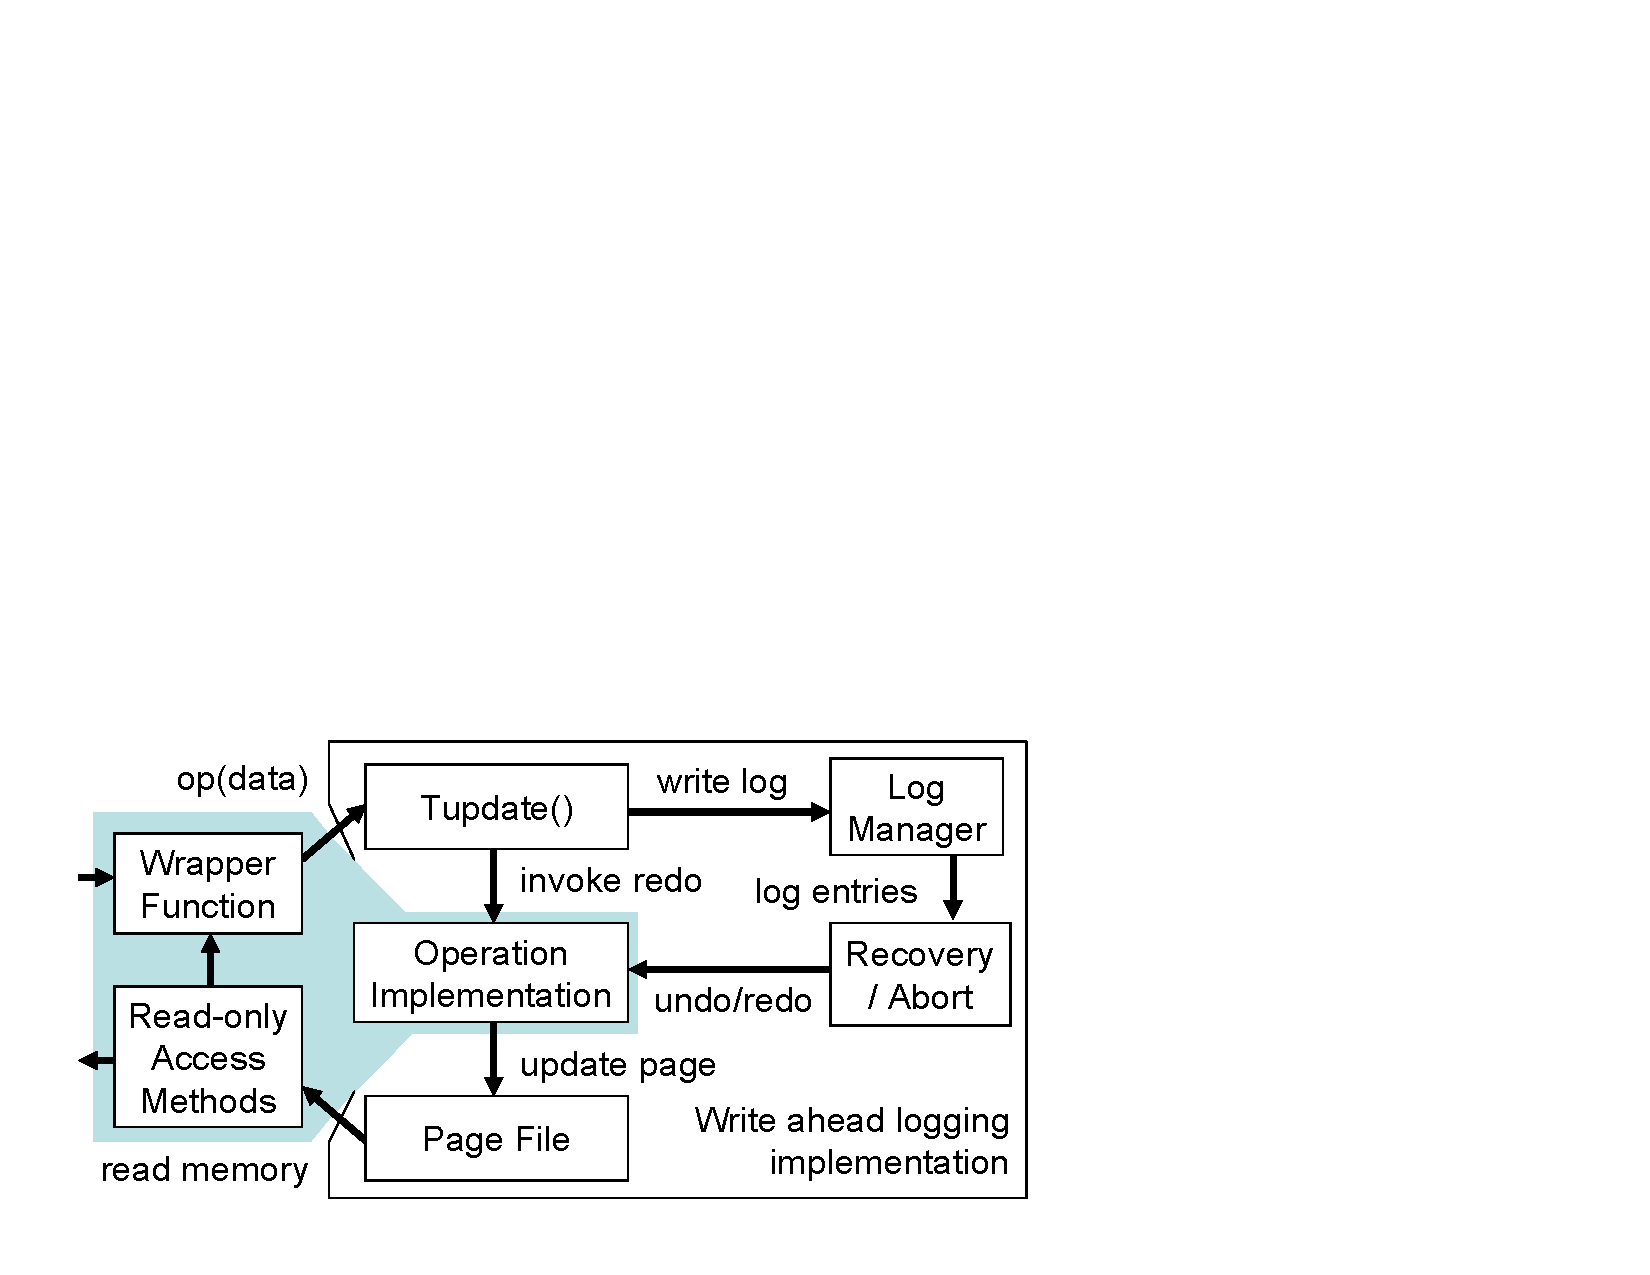
\includegraphics[%
   width=1\columnwidth]{figs/structure.pdf}
\caption{\sf\label{fig:structure} The portions of \yad that new operations directly interact with.}
\end{figure}
\yad allows application developers to easily add new operations to the
system.  Many of the customizations described below can be implemented
using custom log operations.  In this section, we desribe how to add a
``typical'' Steal/no-Force operation that supports concurrent
transactions, full physiological logging, and per-page LSN's.  Such
opeartions are typical of high-performance commercial database
engines.

As we mentioned above, \yad operations must implement a number of
functions.  Figure~\ref{yadArch} describes the environment that
schedules and invokes these functions.  The first step in implementing
a new set of log interfaces is to decide upon interface that these log
interfaces will export to callers outside of \yad.  

These interfaces are implemented by the Wrapper Functions and Read
only access methods in Figure~\ref{yadArch}.  Wrapper functions that
modify the state of the database package any information that will be
needed for undo or redo into a data format of its choosing.  This data
structure, and an opcode associated with the type of the new
operation, are passed into Tupdate(), which copies its arguments to
the log, and then passes its arguments into the operation's REDO
function.
 
REDO modifies the page file, or takes some other action directly.  It
is essentially an iterpreter for the log entries it is associated
with.  UNDO works analagously, but is invoked when an operation must
be undone (usually due to an aborted transaction, or during recovery).
This general pattern is quite general, and applies in many cases.  In
order to implement a ``typical'' operation, the operations
implementation must obey a few more invariants:

\begin{itemize}
\item Pages should only be updated inside REDO and UNDO functions.
\item Page updates atomically update page LSN's by pinning the page.
\item If the data seen by a wrapper function must match data seen
  during REDO, then the wrapper should use a latch to protect against
  concurrent attempts to update the sensitive data (and against
  concurrent attempts to allocate log entries that update the data).
\item Nested top actions (and logical undo), or ``big locks'' (which
  reduce concurrency) should be used to implement multi-page updates.
\end{itemize}

\subsection{Linear hash table}
\begin{figure}[t]
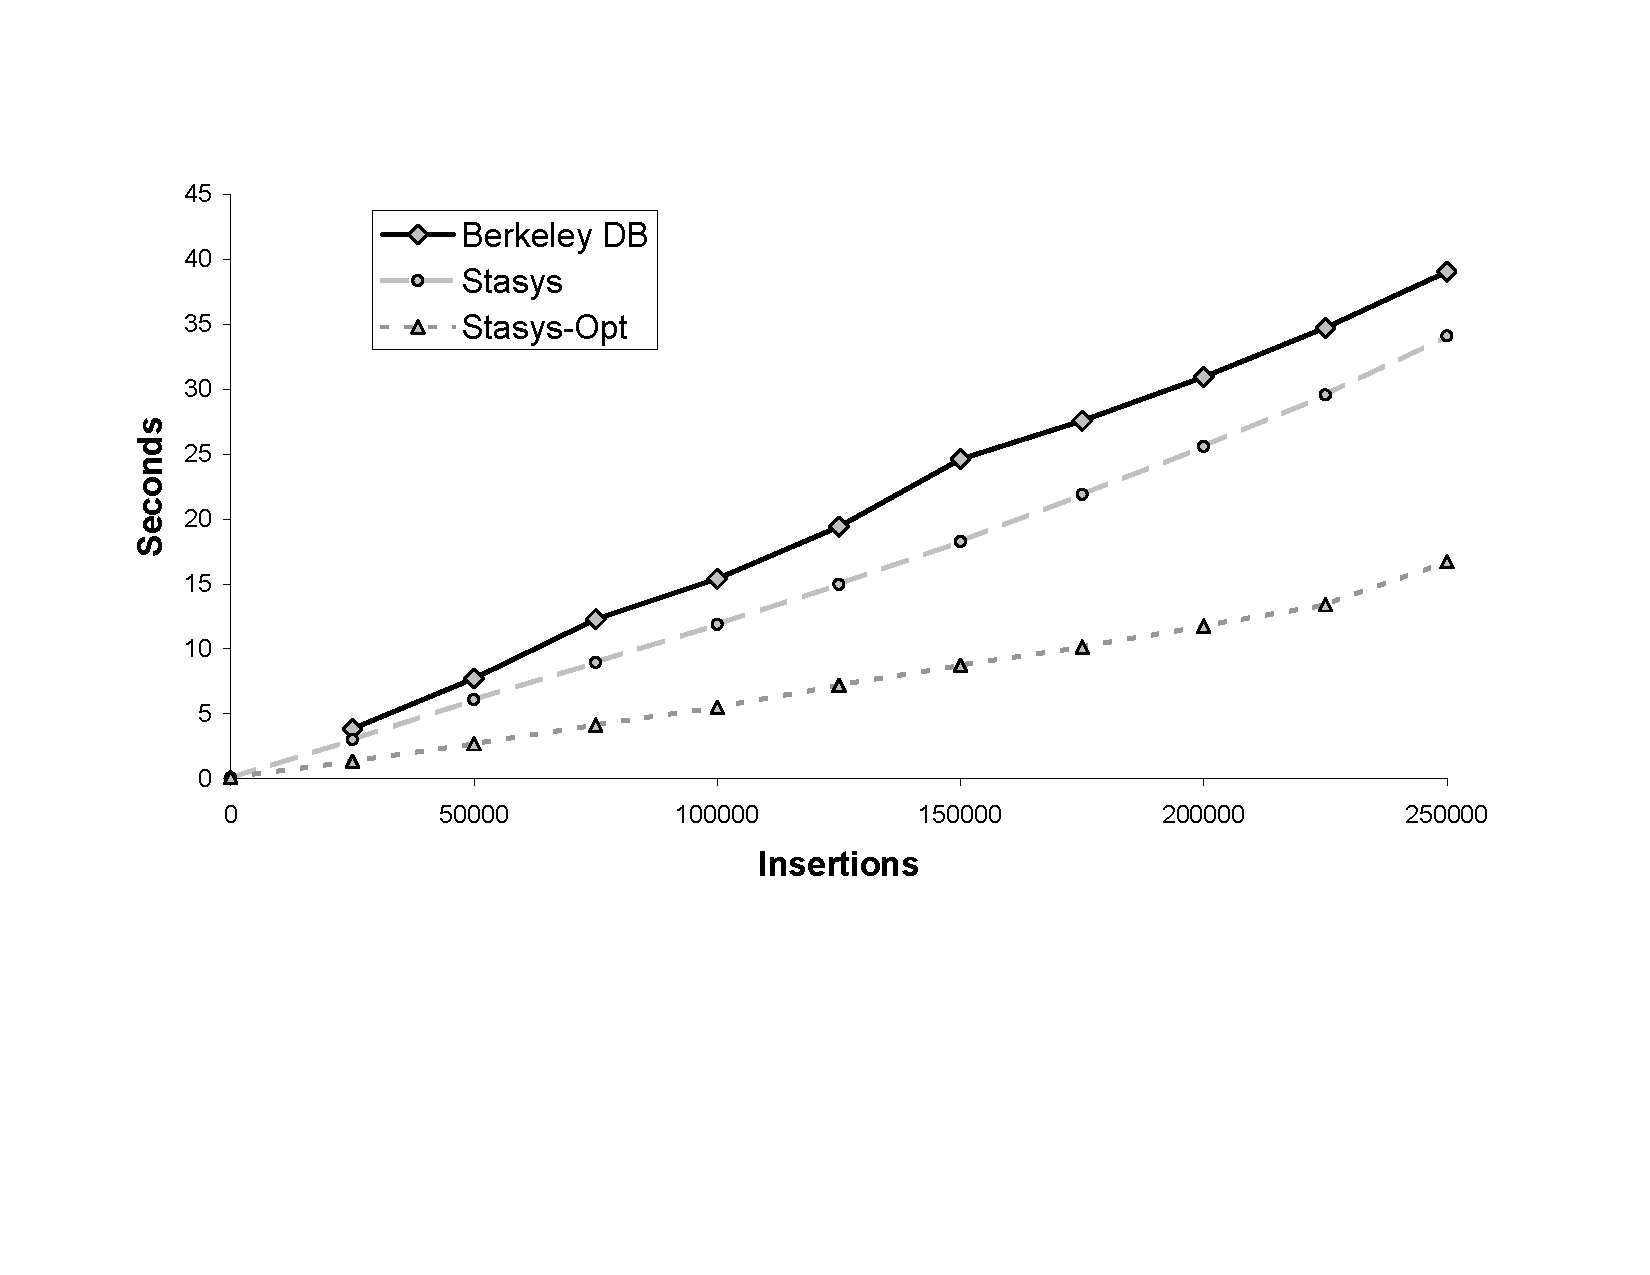
\includegraphics[%
   width=1\columnwidth]{figs/bulk-load.pdf}
%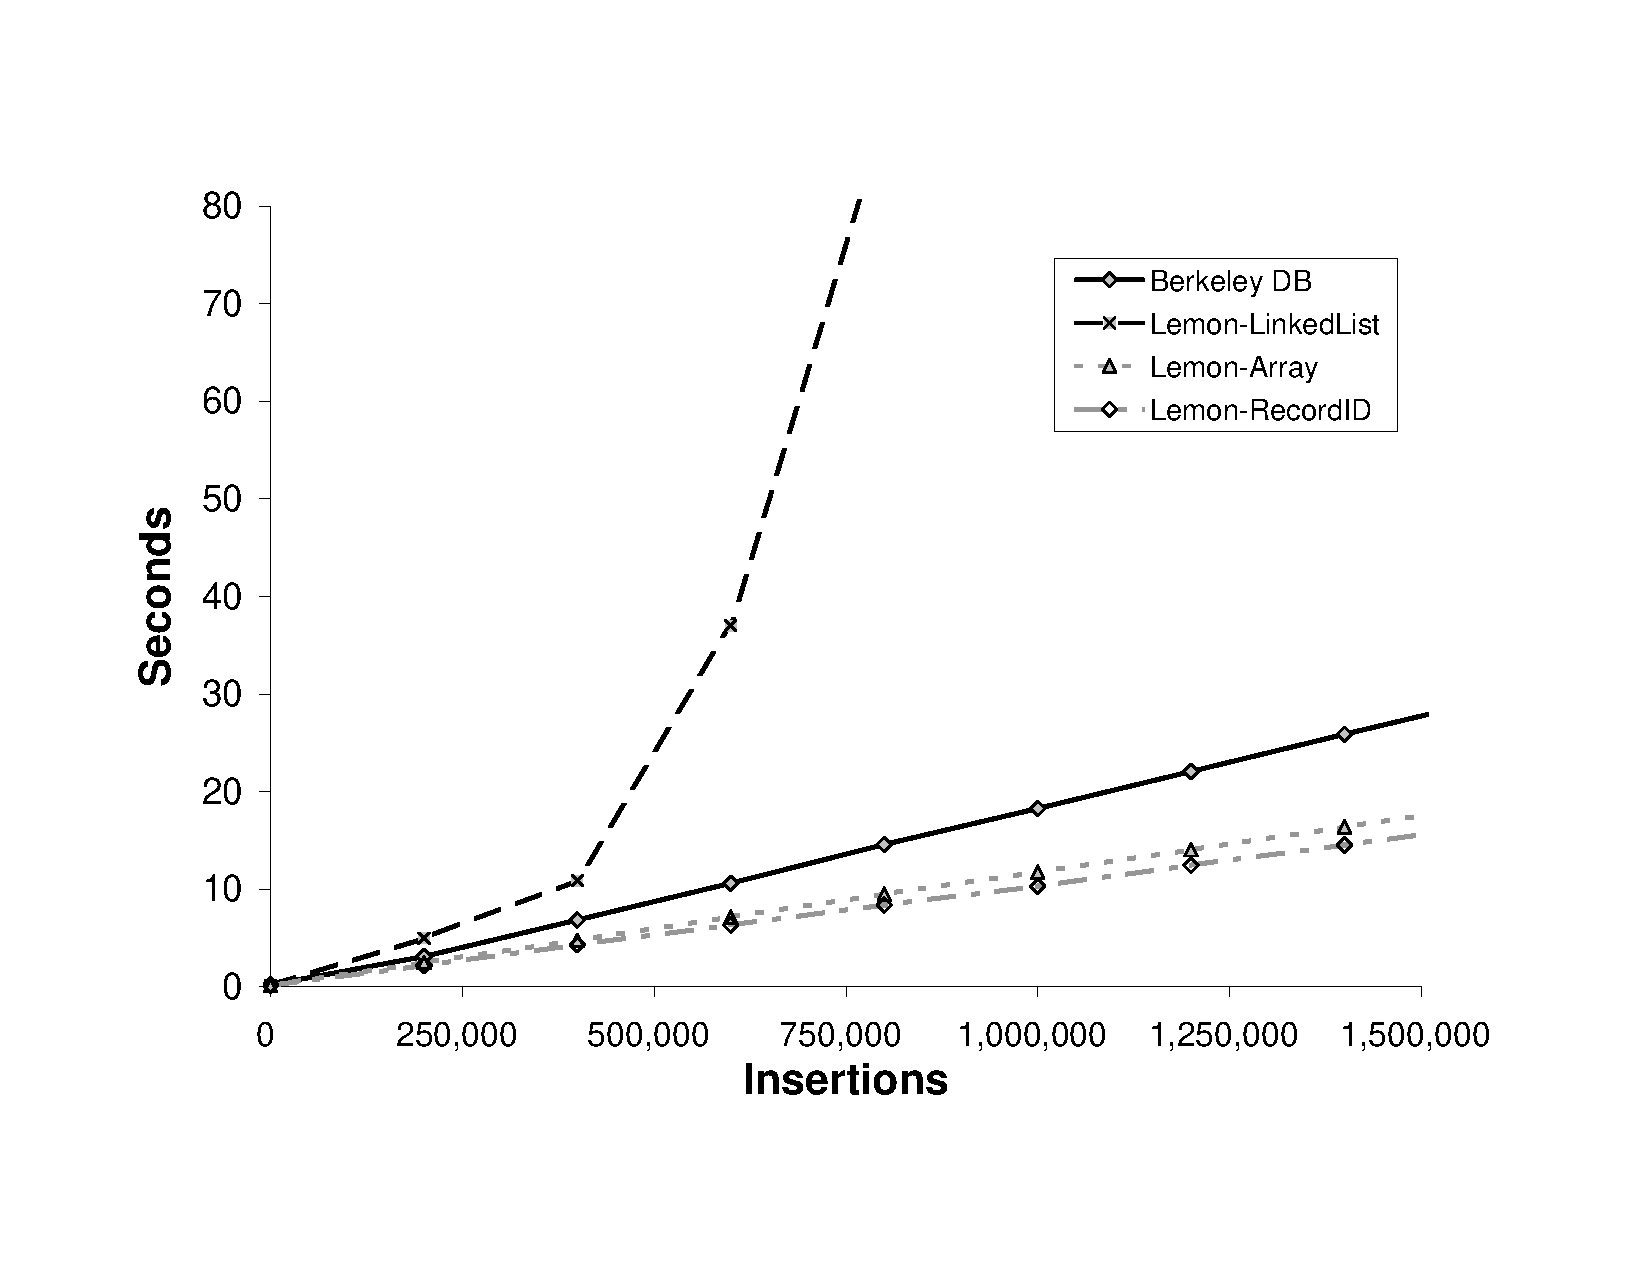
\includegraphics[%
%   width=1\columnwidth]{bulk-load-raw.pdf}
%\vspace{-30pt}
\caption{\sf\label{fig:BULK_LOAD} Performance of \yad and Berkeley DB hashtable implementations.  The
test is run as a single transaction, minimizing overheads due to synchronous log writes.}
\end{figure}
\begin{figure}[t]
%\hspace*{18pt}
%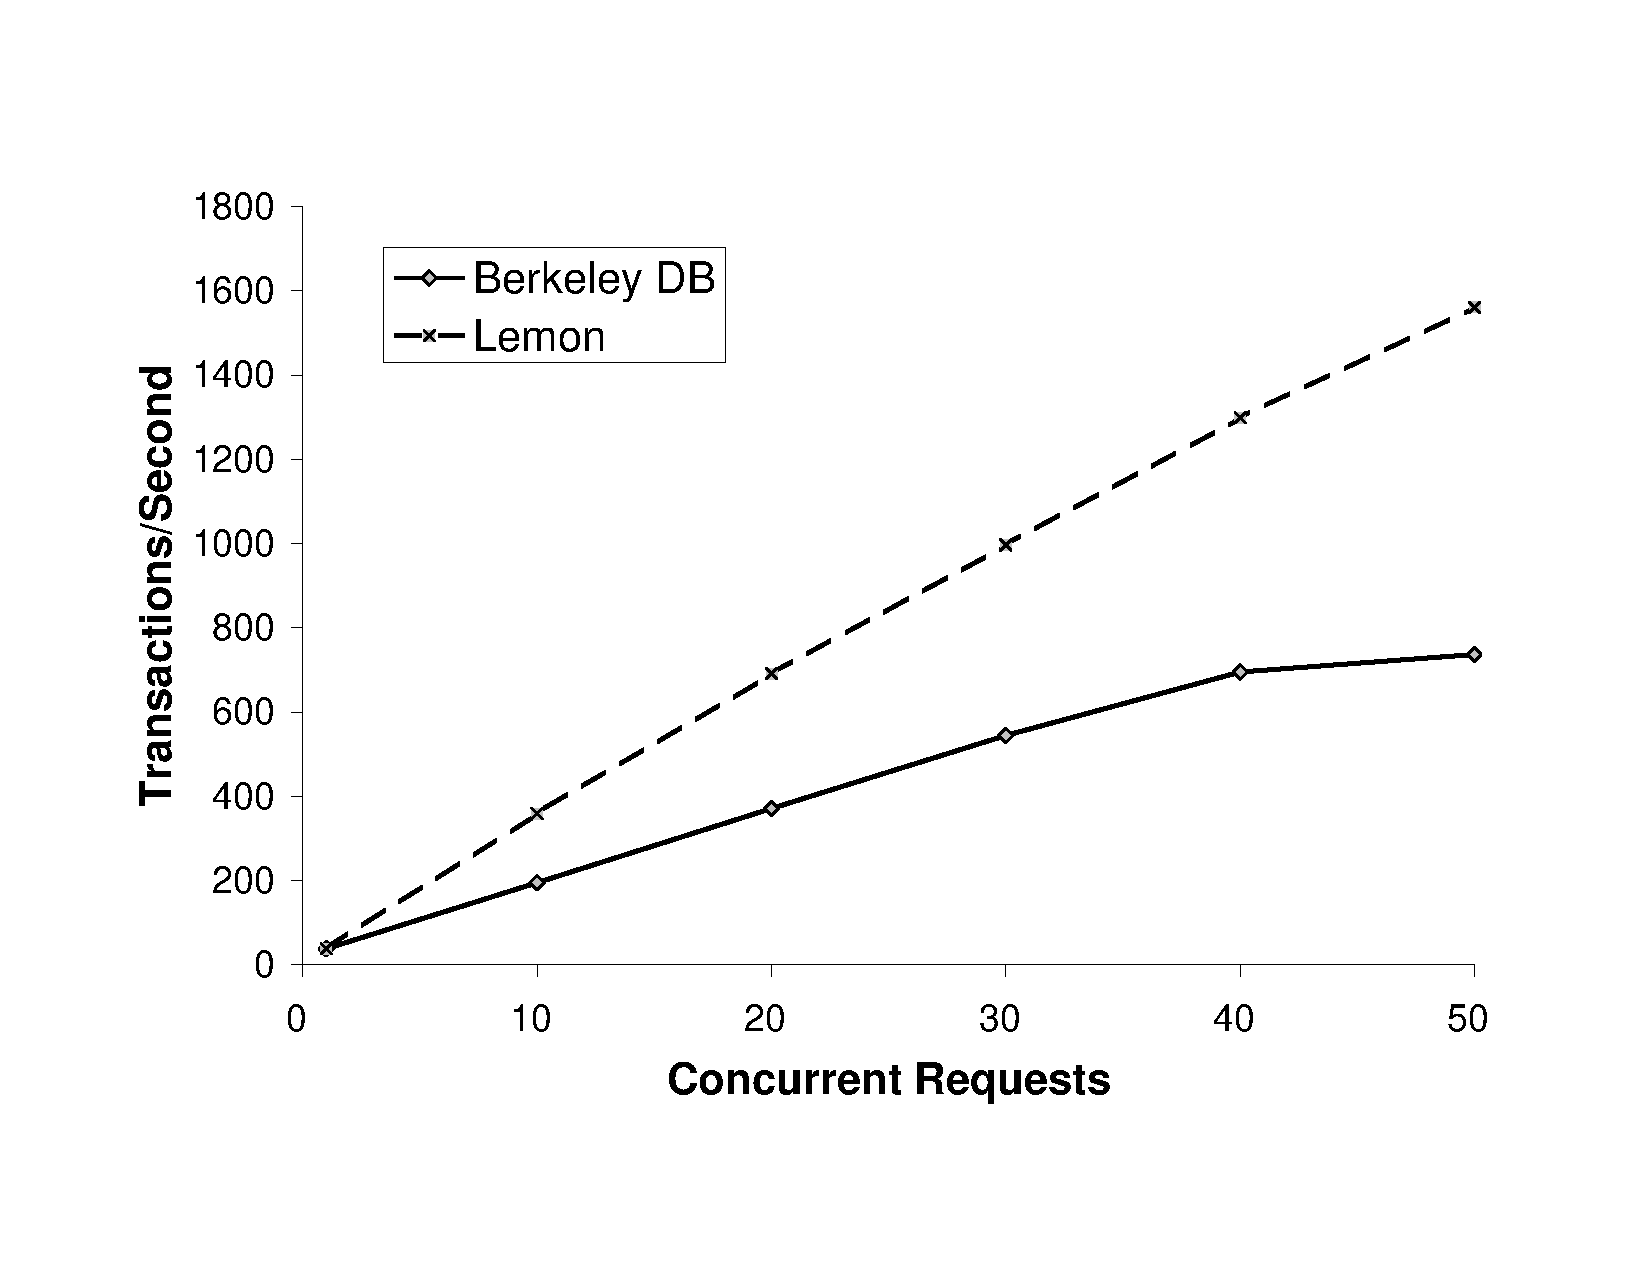
\includegraphics[%
%   width=1\columnwidth]{tps-new.pdf}
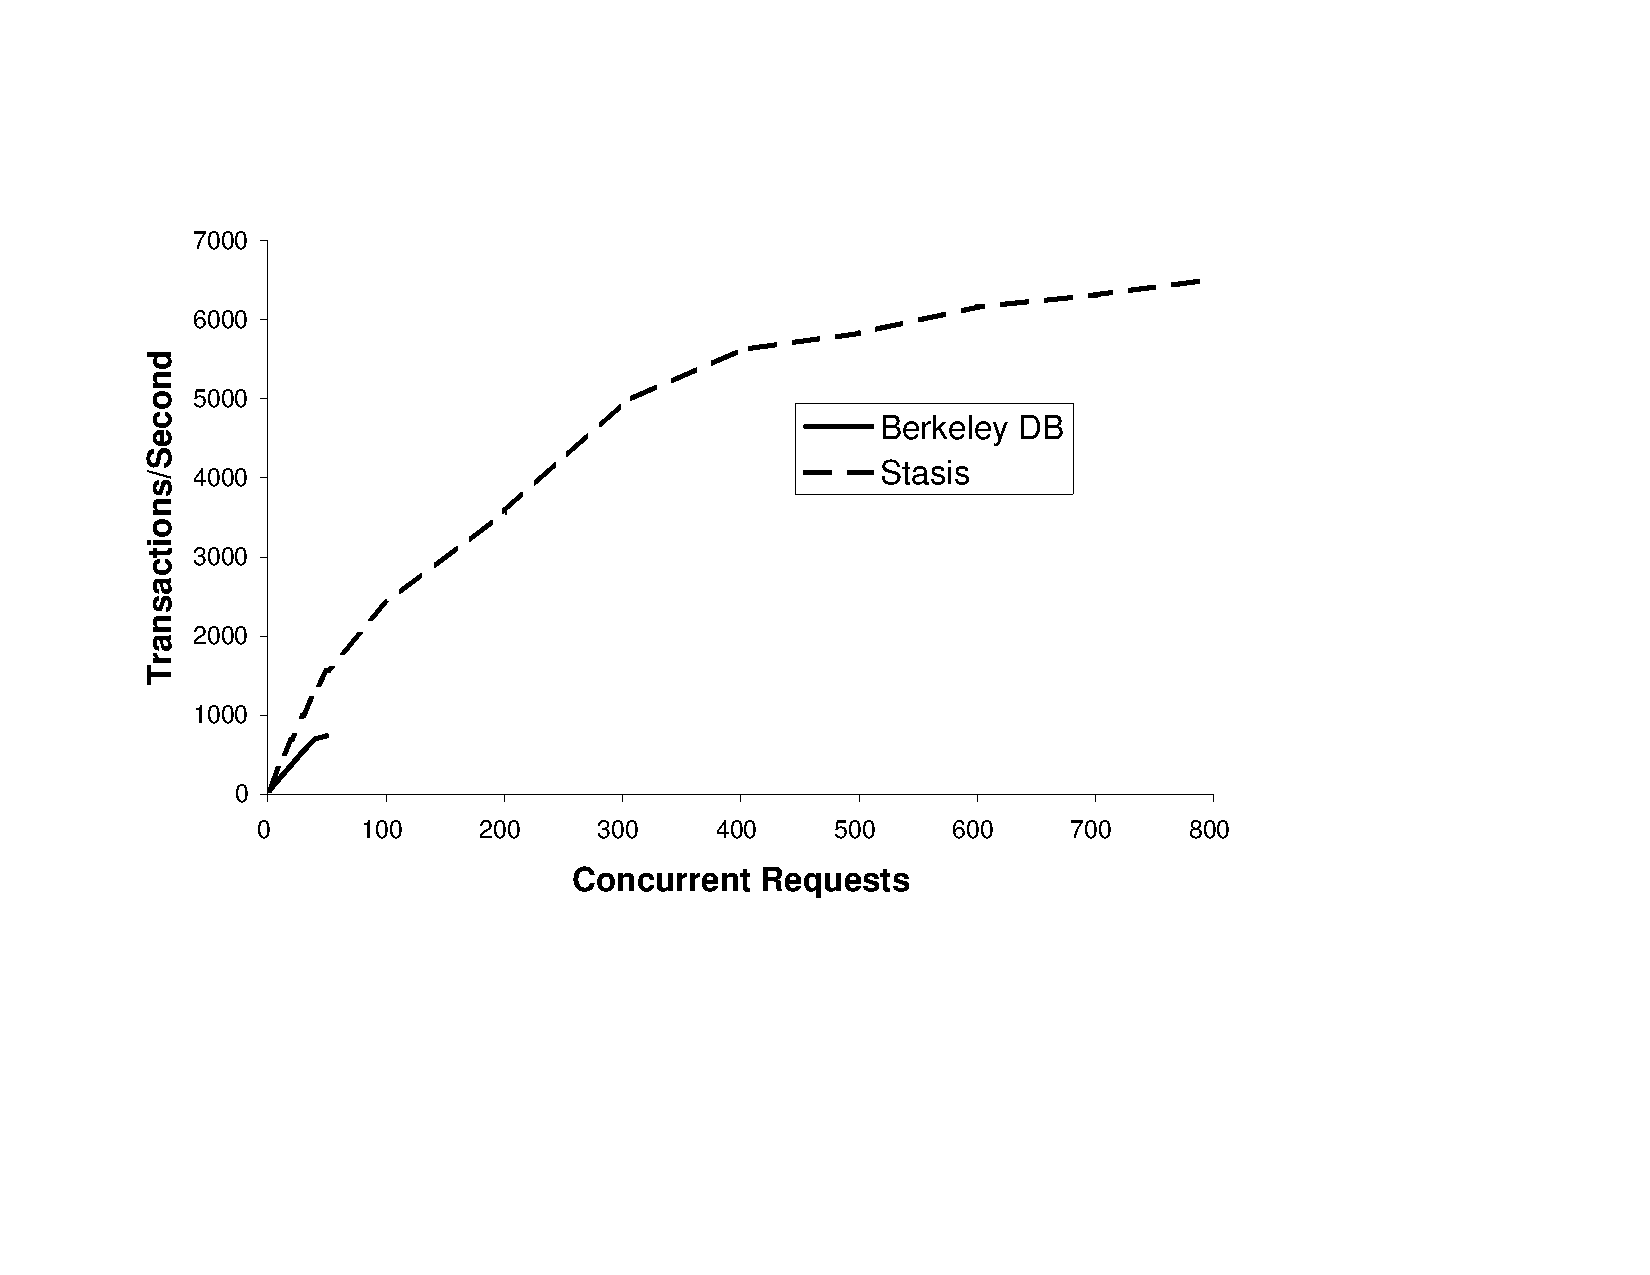
\includegraphics[%
   width=3.25in]{figs/tps-extended.pdf}
%\vspace{-36pt}
\caption{\sf\label{fig:TPS} High concurrency performance of Berkeley DB and \yad.  We were unable to get Berkeley DB to work correctly with more than 50 threads. (See text)
}
\end{figure}

Although the beginning of this paper describes the limitations of
physical database models and relational storage systems in great
detail, these systems are the basis of most common transactional
storage routines.  Therefore, we implement key-based storage, and a
primititve form of linksets in this section.  We argue that obtaining
obtaining reasonable performance in such a system under \yad is
straightforward, and compare a simple hash table to a hand-tuned (not
straightforward) hash table, and Berkeley DB's implementation.

The simple hash table uses nested top actions to atomically update its
internal structure.  It is based on a linear hash function, allowing
it to incrementally grow its buffer list.  It is based on a number of
modular subcomponents, notably a growable array of fixed length
entries, and the user's choice of two different linked list
implementations.  The hand-tuned hashtable also uses a {\em linear} hash
function,~\cite{lht} but is monolithic, and uses carefully ordered writes to
reduce log bandwidth, and other runtime overhead.  Berkeley DB's
hashtable is a popular, commonly deployed implementation, and serves
as a baseline for our experiements.

Both of our hashtables outperform Berkeley DB on a workload that
bulkloads the tables by repeatedly inserting key, value pairs into
them.  We do not claim that our partial implementation of \yad
generally outperforms Berkeley DB, or that it is a robust alternative
to Berkeley DB.  Instead, this test shows that \yad is comparable to
existing systems, and that its modular design does not introduce gross
inefficiencies at runtime.

The comparison between our two hash implementations is more
enlightening.  The performance of the simple hash table shows that
quick, straightfoward datastructure implementations composed from
simpler structures behave reasonably well in \yad.  The hand-tuned
implementation shows that \yad allows application developers to
optimize the primitives they build their applications upon.  In the
best case, past systems allowed application developers to providing
hints to improve performance.  In the worst case, a developer would be
forced to redesign the application to avoid sub-optimal properties of
the transactional data structure implementation.

Figure~\ref{lhtThread} describes performance of the two systems under
highly concurrent workloads.  For this test, we used the simple
(unoptimized) hash table, since we are interested in the performance a
clean, modular data structure that a typical system implementor would
be likely to produce, not the performance of our own highly tuned,
monolithic, implementations.

Both Berekely DB and \yad can service concurrent calls to commit with
a single synchronous I/O.\endnote{The multi-threaded benchmarks
  presented here were performed using an ext3 filesystem, as high
  concurrency caused both Berkeley DB and \yad to behave unpredictably
  when reiserfs was used.  However, \yads multi-threaded throughput
  was significantly better that Berkeley DB's under both systems.}
\yad scaled quite well, delivering over 6000 transactions per
second,\endnote{This test was run without lock managers, so the
  transactions obeyed the A, C, and D properties.  Since each
  transaction performed exactly one hashtable write and no reads, they
  obeyed I (isolation) in a trivial sense.}  and provided roughly
double Berkeley DB's throughput (up to 50 threads).  We do not report
the data here, but we implemented a simple load generator that makes
use of a fixed pool of threads with a fixed think time.  We found that
the latency of Berkeley DB and \yad were similar, addressing concerns
that \yad simply trades latency for throughput during the concurrency
benchmark.

\subsection{Object serialization}

\begin{figure*}[t!]
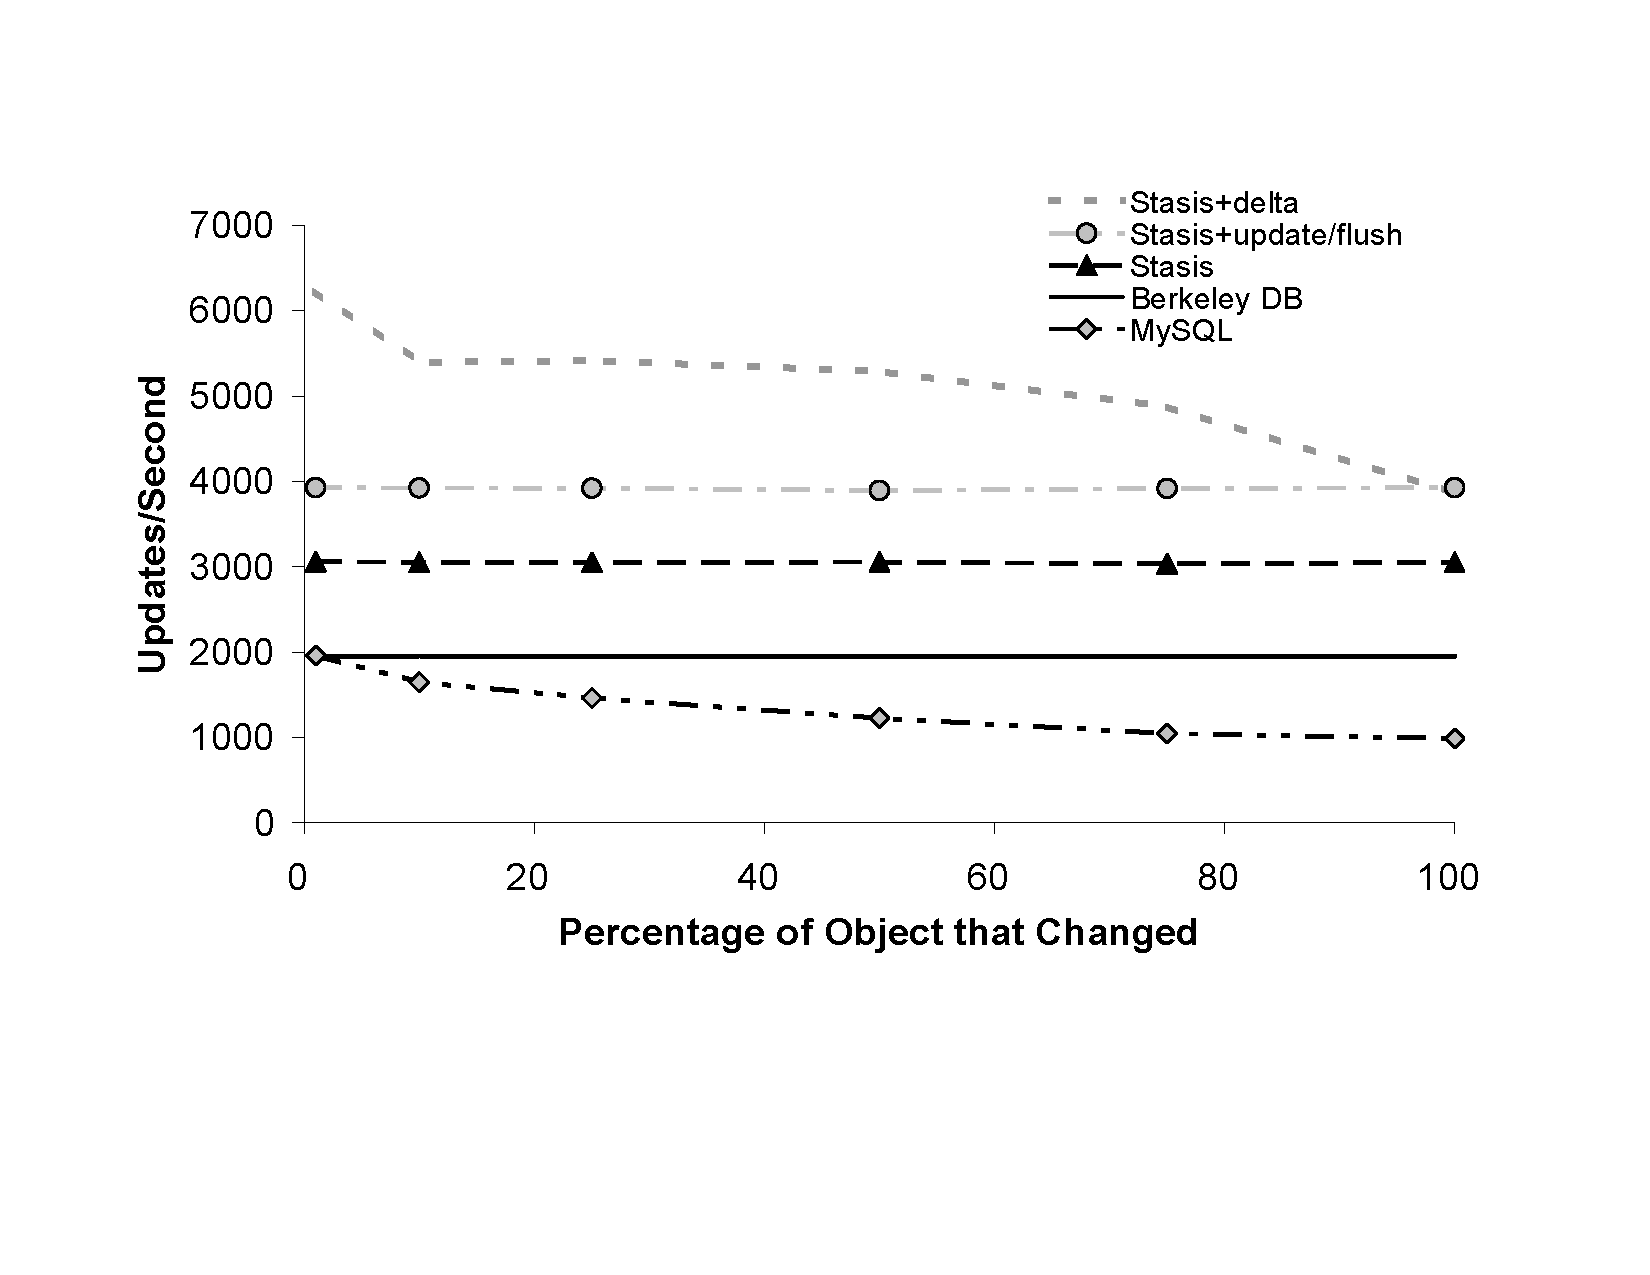
\includegraphics[width=3.3in]{figs/object-diff.pdf}
\hspace{.3in}
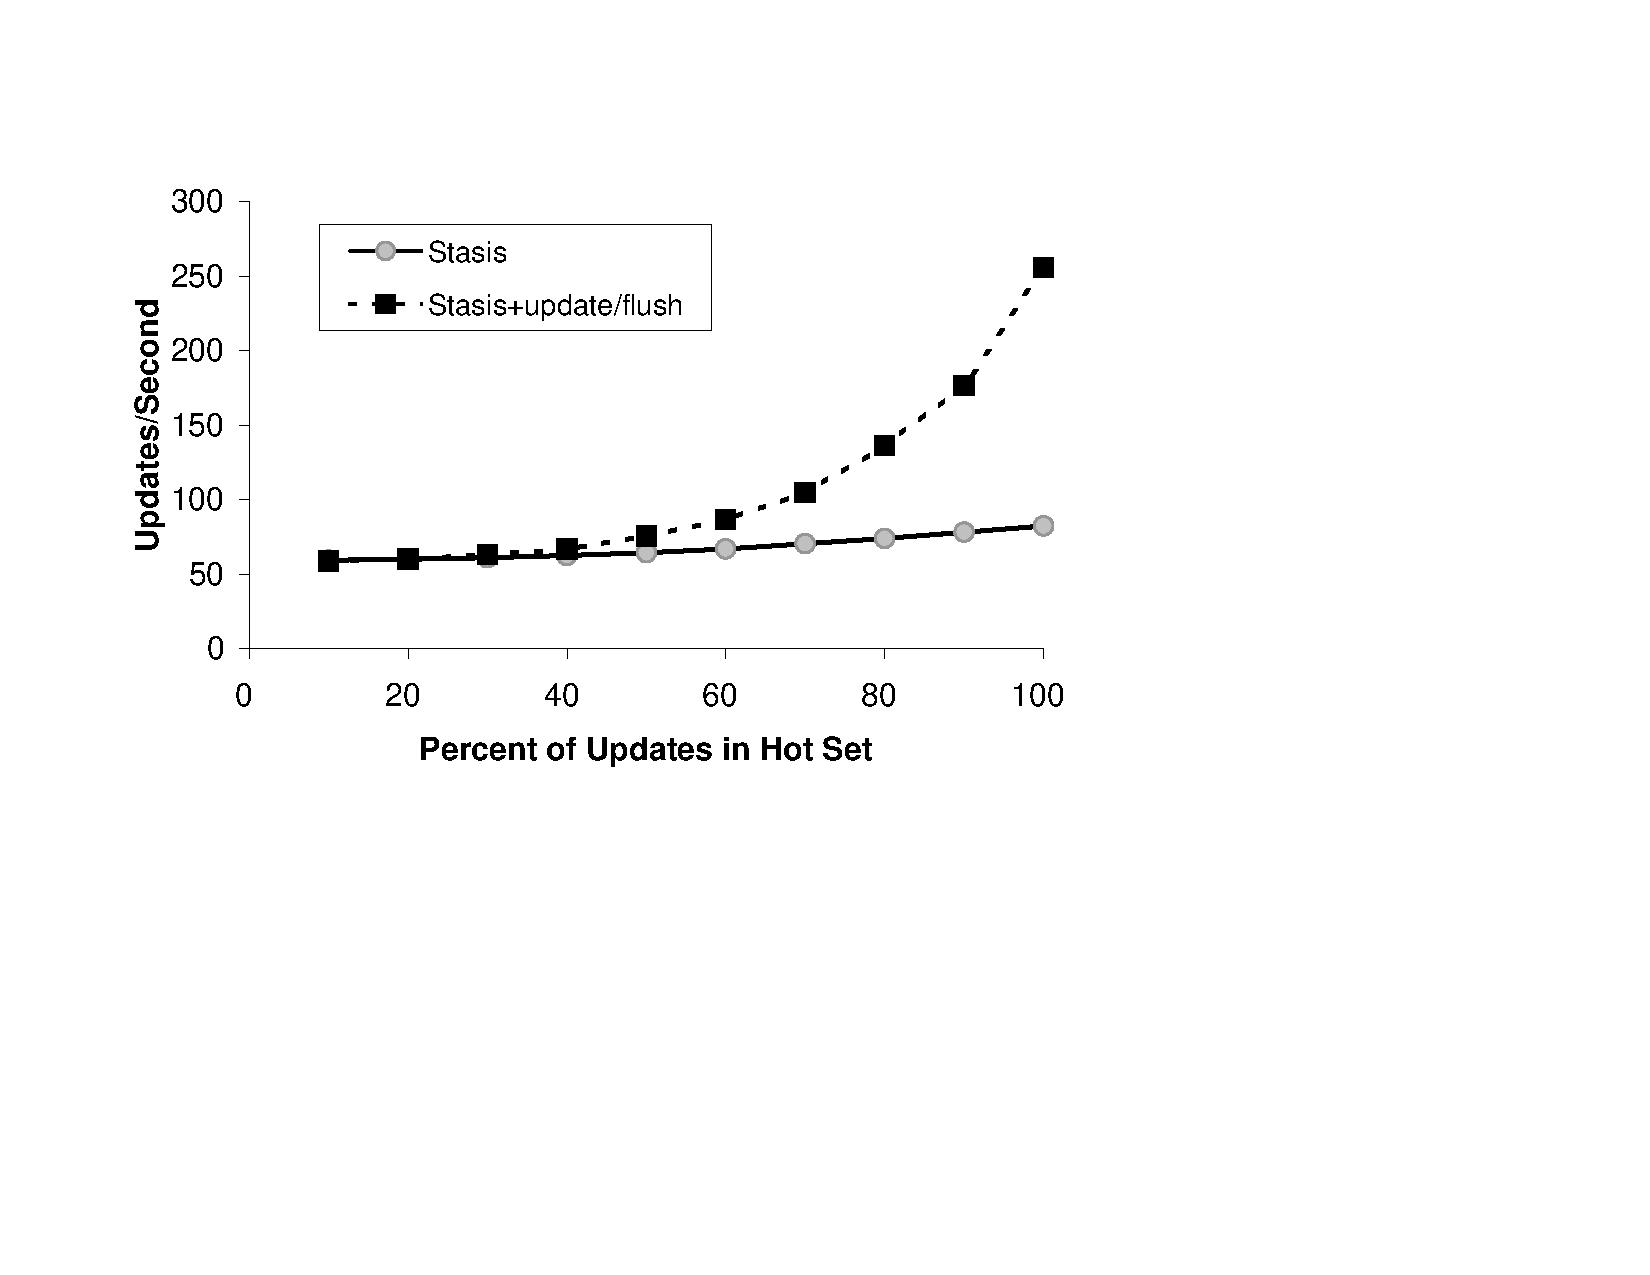
\includegraphics[width=3.3in]{figs/mem-pressure.pdf}
\vspace{-.15in}
\caption{\sf \label{fig:OASYS}
The effect of \yad object serialization optimizations under low and high memory pressure.}
\end{figure*}

\subsection{Object persistance mechanisms}
\rcs{ This belongs somewhere else: Instead, it leaves decisions regarding abstract data types and
algorithm design to system developers or language designers.  For
instance, while \yad has no concept of object oriented data types, two
radically different approaches toward object persistance have been
implemented on top of it~\ref{oasys}.}

\rcs{We could have just as easily written a persistance mechanism for a
functional programming language, or a particular application (such as
an email server).  Our experience building data manipulation routines
on top of application-specific primitives was favorable compared to
past experiences attempting to restructure entire applications to
match pre-existing computational models, such as SQL's declarative
interface.}




Numerous schemes are used for object serialization.  Support for two
different styles of object serialization have been eimplemented in
\yad.  The first, pobj, provided transactional updates to objects in
Titanium, a Java variant.  It transparently loaded and persisted
entire graphs of objects.

The second variant was built on top of a generic C++ object
serialization library, \oasys.  \oasys makes use of pluggable storage
modules to actually implement persistant storage, and includes plugins
for Berkeley DB and MySQL.  This section will describe how the \yads
\oasys plugin reduces the runtime serialization/deserialization cpu
overhead of write intensive workloads, while using half as much system
memory as the other two systems.

We present three variants of \yad here.  The first treats \yad like
Berkeley DB.  The second customizes the behavior of the buffer
manager.  Instead of maintaining an up-to-date version of each object
in the buffer manager or page file, it allows the buffer manager's
view of live application objects to become stale.  This is safe since
the system is always able to reconstruct the appropriate page entry
form the live copy of the object.

The reason it would be difficult to do this with Berkeley DB is that
we still need to generate log entries as the object is being updated.
Otherwise, commit would not be durable, and the application would be
unable to abort() transactions.  Even if we decided to disallow
application aborts, we would still need to write log entries
committing.  This would cause Berekley DB to write data back to the
page file, increasing the working set of the program, and increasing
disk activity.

Under \yad, we implemented this optimization by adding two new
operations, update(), which only updates the log, and flush(), which
updates the page file.  We decrease the size of the page file, so
flush() is likely to incur disk overhead.  However, we have roughly
doubled the number of objects that are cached in memory, and expect
flush() to be called relatively infrequently.

The third \yad plugin to \oasys incorporated all of the updates of the
second, but arranged to only the changed portions of objects to the
log.

Figure~\ref{objectSerialization} presents the performance of the three
\yad optimizations, and the \oasys plugins implemented on top of other
systems.  As we can see, \yad performs better than the baseline
systems.  More interestingly, in non-memory bound systems, the
optimizations nearly double \yads performance, and we see that in the
memory-bound setup, update/flush indeed improves memory utilization.


\subsection{Manipulation of logical log entries}

\begin{figure}
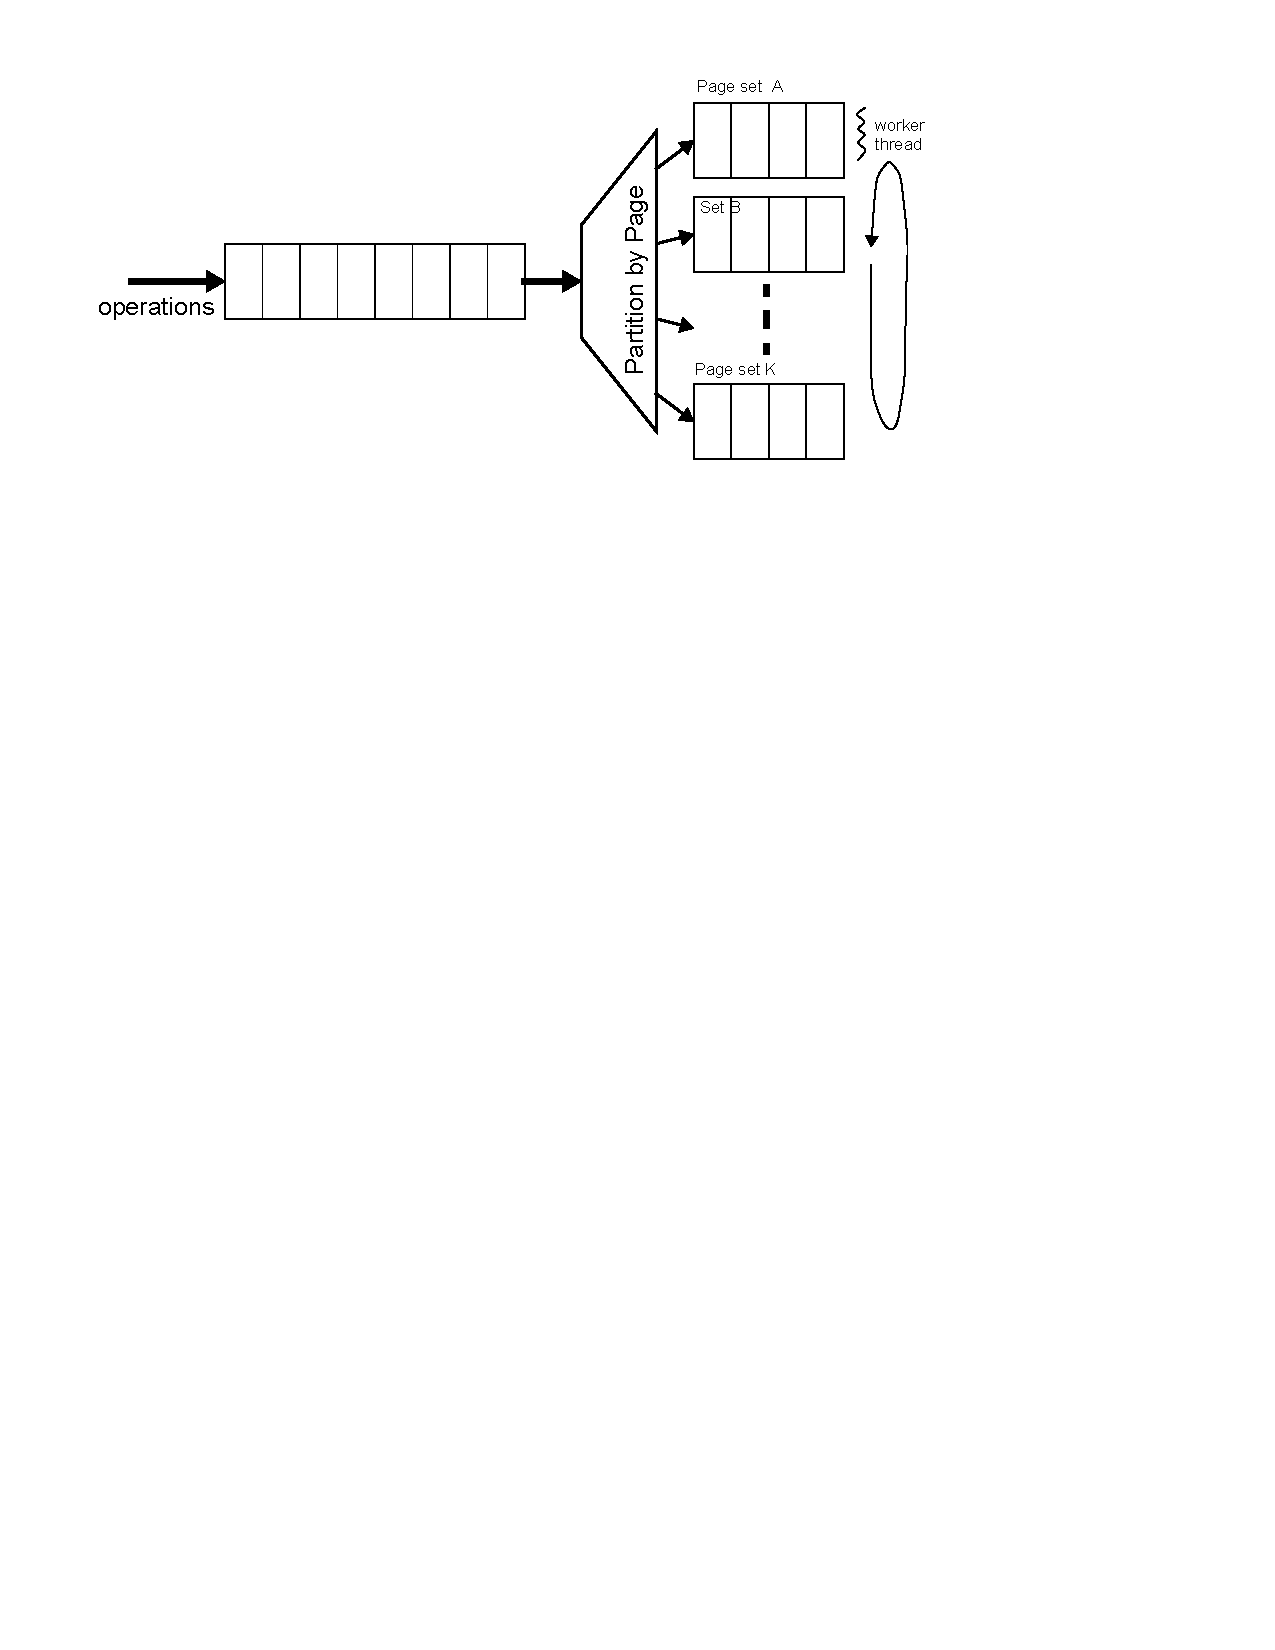
\includegraphics[width=1\columnwidth]{figs/graph-traversal.pdf}
\vspace{-24pt}
\caption{\sf\label{fig:multiplexor} Because pages are independent, we
can reorder requests among different pages. Using a log demultiplexer,
we partition requests into independent queues, which can be 
handled in any order, improving locality and merging opportunities.}
\end{figure}
\begin{figure}[t]
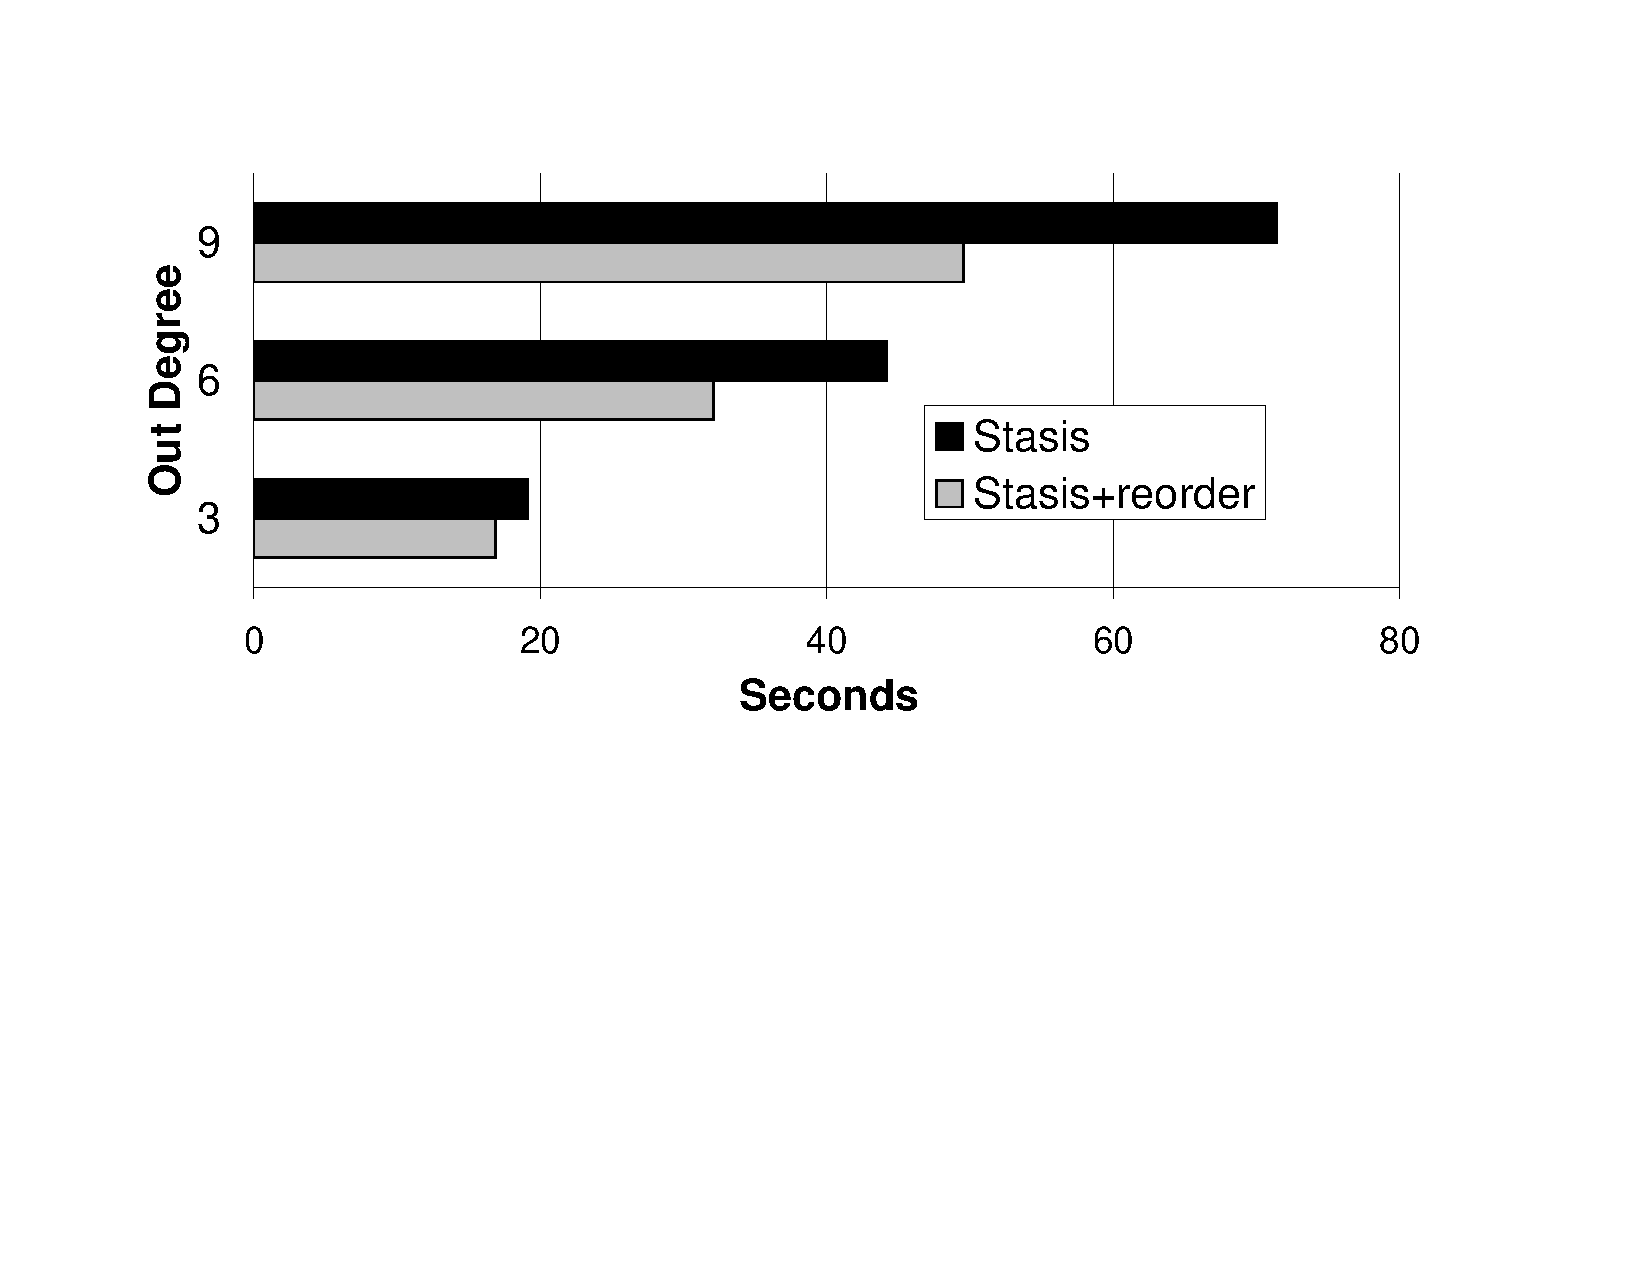
\includegraphics[width=3.3in]{figs/oo7.pdf}
\vspace{-15pt}
\caption{\sf\label{fig:oo7} oo7 benchmark style graph traversal.  The optimization performs well due to the presence of non-local nodes.}
\end{figure}

\begin{figure}[t]
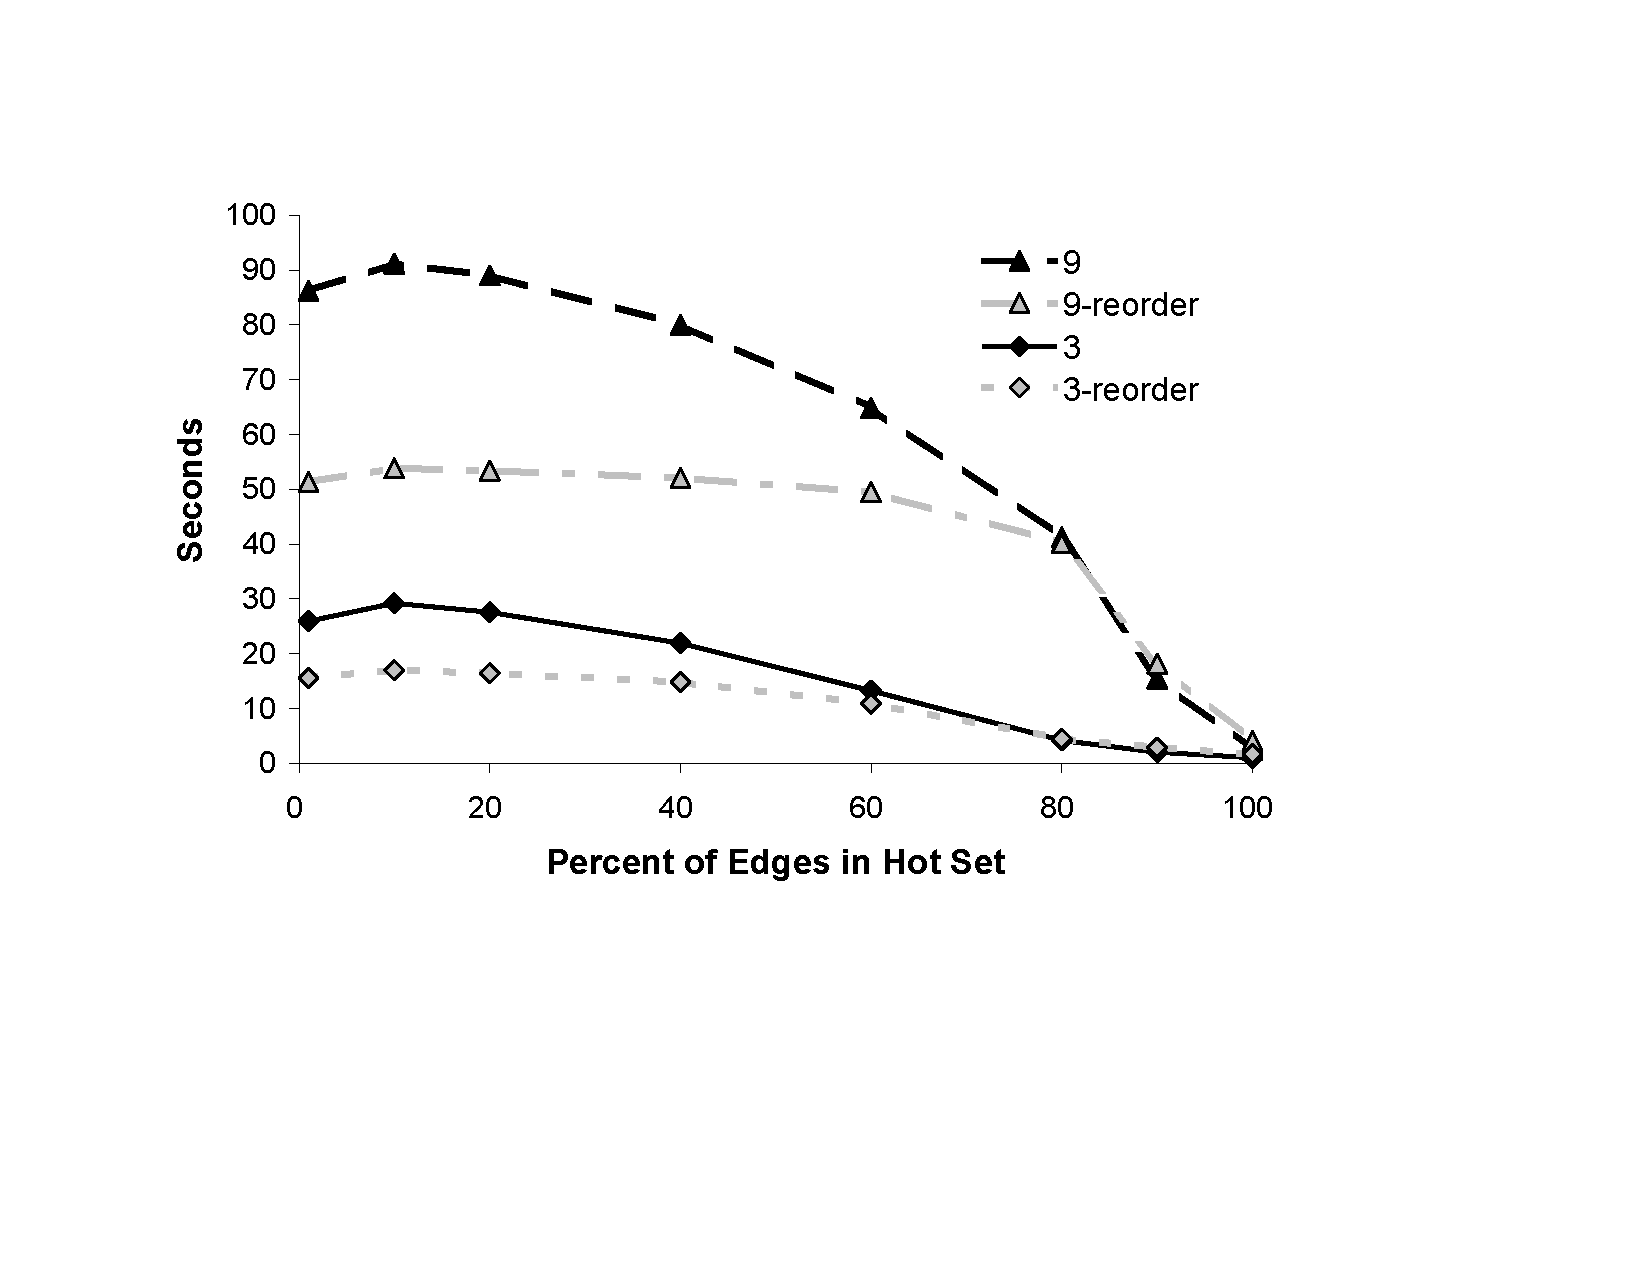
\includegraphics[width=3.3in]{figs/trans-closure-hotset.pdf}
\vspace{-12pt}
\caption{\sf\label{fig:hotGraph} Hot set based graph traversal for random graphs with out-degrees of 3 and 9.  Here
we see that the multiplexer helps when the graph has poor locality.
However, in the cases where depth first search performs well, the
reordering is inexpensive.}
\end{figure}

Database optimizers operate over relational algebra expressions that
will correspond to sequence of logical operations at runtime.  \yad
does not support query languages, relational algebra, or other general
purpose primitves.

However, it does include an extendible logging infrastructure, and any
operations that make user of physiological logging implicitly
implement UNDO (and often REDO) functions that interpret logical
operations.

Logical operations often have some nice properties that this section
will exploit.  Because they can be invoked at arbitrary times in the
future, they tend to be independent of the database's physical state.
They tend to be inverses of operations that programmer's understand.
If each method in the API exposed to the programmer is the inverse of
some other method in the API, then each logical operation corresponds
to a method the programmer can manually invoke.

Because of this, application developers can easily determine whether
logical operations may safely be reordered, transformed, or even
dropped from the stream of requests that \yad is processing.  Even
better, if requests can be partitioned in a natural way, load
balancing can be implemented by spliting requests across many nodes.
Similarly, a node can easily service streams of requests from multiple
nodes by combining them into a single log, and processing the log
using operaiton implementations.  Furthermore, application-specific
procedures that are analagous to standard relational algebra methods
(join, project and select) could be used to efficiently transform the data
before it reaches the page file, while it is layed out sequentially
in memory.

Note that read-only operations do not necessarily generate log
entries.  Therefore, applications may need to implement custom
operations to make use of the ideas in this section.

Although \yad has rudimentary support for a two-phase commit based
cluster hash table, we have not yet implemented a logical log based
networking primitives.  Therefore, we implemented some of these ideas
in a single node configuration in order to increase request locality
during the traversal of a random graph.  The graph traversal system
takes a sequence of (read) requests, and partitions them using some
function.  It then proceses each partition in isolation from the
others.  We considered two partitioning functions.  The first, which
is really only of interested in the distributed case, partitions the
requests according to the hash of the node id they refer to.  This
would allow us to balance the graph traversal across many nodes.  (We
expect the early phases of such a traversal to be bandwidth, not
latency limited, as each node would stream large sequences of
asynchronous requests to the other nodes.) 

The second partitioning function, which was used to produce
Figure~\ref{hotset} partitions requests by their position in the page
file.  When the graph has good locality, a normal depth first search
traversal and the prioritized traversal perform well.  As locality
decreases, the partitioned traversal algorithm's performance degrades
less than the naive traversal.

**TODO This really needs more experimental setup... look at older draft!**

\subsection{LSN-Free pages}

In Section~\ref{todo}, we describe how operations can avoid recording
LSN's on the pages they modify.  Essentially, opeartions that make use
of purely physical logging need not heed page boundaries, as
physiological operations must.  Recall that purely physical logging
interacts poorly with concurrent transactions that modify the same
data structures or pages, so LSN-Free pages are not applicable in all
situations.

Consider the retreival of a large (page spanning) object stored on
pages that contain LSN's.  The object's data will not be contiguous.
Therefore, in order to retrive the object, the transaction system must
load the pages contained on disk into memory, allocate buffer space to
allow the object to be read, and perform a byte-by-byte copy of the
portions of the pages that contain the large object's data.  Compare
this approach to a modern filesystem, which allows applications to
perform a DMA copy of the data into memory, avoiding the expensive
byte-by-byte copy of the data, and allowing the CPU to be used for
more productive purposes.  Furthermore, modern operating systems allow
network services to use DMA and ethernet adaptor hardware to read data
from disk, and send it over a network socket without passing it
through the CPU.  Again, this frees the CPU, allowing it to perform
other tasks.

We beleive that LSN free pages will allow reads to make use of such
optimizations in a straightforward fashion.  Zero copy writes could be
performed by performing a DMA write to a portion of the log file.
However, doing this complicates log truncation, and does not address
the problem of updating the page file.  We suspect that contributions
from the log based filesystem literature can address these problems in
a straightforward fashion.

Finally, RVM, recoverable virtual memory, made use of LSN-free pages
so that it could use mmap() to map portions of the page file into
application memory.  However, without support for logical log entries
and nested top actions, it would be difficult to implement a
concurrent, durable data structure using RVM.  We plan to add RVM
style transactional memory to \yad in a way that is compatible with
fully concurrent collections such as hash tables and tree structures.


\section{Related Work?}

The Boxwood system provides a networked, fault-tolerant transactional
B-Tree and ``Chunk Manager.''  We believe that \yad is an interesting
complement to such a system, especially given \yads focus on
intelligence and optimizations within a single node, and Boxwoods
focus on multiple node systems.  In particular, when implementing
applications with predictable locality properties, it would be
interesting to explore extensions to the Boxwood approach that make
use of \yads customizable semantics (Section~\ref{wal}), and fully logical logging
mechanism. (Section~\ref{logging})

\section{Conclusion}

\section{Acknowledgements}

mike demmer, others?

\section{Availability}

Additional information, and \yads source code is available at:

\begin{center}
{\tt http://\yad.sourceforge.net/}
\end{center}

{\footnotesize \bibliographystyle{acm}
\nocite{*}
\bibliography{LLADD}}

\theendnotes

\end{document}







